\documentclass[man]{apa6}
\usepackage{lmodern}
\usepackage{amssymb,amsmath}
\usepackage{ifxetex,ifluatex}
\usepackage{fixltx2e} % provides \textsubscript
\ifnum 0\ifxetex 1\fi\ifluatex 1\fi=0 % if pdftex
  \usepackage[T1]{fontenc}
  \usepackage[utf8]{inputenc}
\else % if luatex or xelatex
  \ifxetex
    \usepackage{mathspec}
  \else
    \usepackage{fontspec}
  \fi
  \defaultfontfeatures{Ligatures=TeX,Scale=MatchLowercase}
\fi
% use upquote if available, for straight quotes in verbatim environments
\IfFileExists{upquote.sty}{\usepackage{upquote}}{}
% use microtype if available
\IfFileExists{microtype.sty}{%
\usepackage{microtype}
\UseMicrotypeSet[protrusion]{basicmath} % disable protrusion for tt fonts
}{}
\usepackage{hyperref}
\hypersetup{unicode=true,
            pdftitle={The development of infants' responses to mispronunciations - A Meta-Analysis},
            pdfauthor={Katie Von Holzen~\& Christina Bergmann},
            pdfkeywords={keywords},
            pdfborder={0 0 0},
            breaklinks=true}
\urlstyle{same}  % don't use monospace font for urls
\usepackage{graphicx,grffile}
\makeatletter
\def\maxwidth{\ifdim\Gin@nat@width>\linewidth\linewidth\else\Gin@nat@width\fi}
\def\maxheight{\ifdim\Gin@nat@height>\textheight\textheight\else\Gin@nat@height\fi}
\makeatother
% Scale images if necessary, so that they will not overflow the page
% margins by default, and it is still possible to overwrite the defaults
% using explicit options in \includegraphics[width, height, ...]{}
\setkeys{Gin}{width=\maxwidth,height=\maxheight,keepaspectratio}
\IfFileExists{parskip.sty}{%
\usepackage{parskip}
}{% else
\setlength{\parindent}{0pt}
\setlength{\parskip}{6pt plus 2pt minus 1pt}
}
\setlength{\emergencystretch}{3em}  % prevent overfull lines
\providecommand{\tightlist}{%
  \setlength{\itemsep}{0pt}\setlength{\parskip}{0pt}}
\setcounter{secnumdepth}{0}
% Redefines (sub)paragraphs to behave more like sections
\ifx\paragraph\undefined\else
\let\oldparagraph\paragraph
\renewcommand{\paragraph}[1]{\oldparagraph{#1}\mbox{}}
\fi
\ifx\subparagraph\undefined\else
\let\oldsubparagraph\subparagraph
\renewcommand{\subparagraph}[1]{\oldsubparagraph{#1}\mbox{}}
\fi

%%% Use protect on footnotes to avoid problems with footnotes in titles
\let\rmarkdownfootnote\footnote%
\def\footnote{\protect\rmarkdownfootnote}

%%% Change title format to be more compact
\usepackage{titling}

% Create subtitle command for use in maketitle
\newcommand{\subtitle}[1]{
  \posttitle{
    \begin{center}\large#1\end{center}
    }
}

\setlength{\droptitle}{-2em}
  \title{The development of infants' responses to mispronunciations - A
Meta-Analysis}
  \pretitle{\vspace{\droptitle}\centering\huge}
  \posttitle{\par}
  \author{Katie Von Holzen\textsuperscript{1,2}~\& Christina
Bergmann\textsuperscript{3,4}}
  \preauthor{\centering\large\emph}
  \postauthor{\par}
  \date{}
  \predate{}\postdate{}

\shorttitle{Mispronunciation Meta-Analysis}
\affiliation{
\vspace{0.5cm}
\textsuperscript{1} Language Development Laboratory, University of Maryland, USA\\\textsuperscript{2} Laboratoire Psychologie de la Perception, Université Paris Descartes\\\textsuperscript{3} Max Planck Institute for Psycholinguistics, Nijmegen, the Netherlands\\\textsuperscript{4} LSCP, Departement d'Etudes Cognitives, ENS, EHESS, CNRS, PSL Research University}
\keywords{keywords\newline\indent Word count: X}
\usepackage{csquotes}
\usepackage{upgreek}
\captionsetup{font=singlespacing,justification=justified}

\usepackage{longtable}
\usepackage{lscape}
\usepackage{multirow}
\usepackage{tabularx}
\usepackage[flushleft]{threeparttable}
\usepackage{threeparttablex}

\newenvironment{lltable}{\begin{landscape}\begin{center}\begin{ThreePartTable}}{\end{ThreePartTable}\end{center}\end{landscape}}

\makeatletter
\newcommand\LastLTentrywidth{1em}
\newlength\longtablewidth
\setlength{\longtablewidth}{1in}
\newcommand{\getlongtablewidth}{\begingroup \ifcsname LT@\roman{LT@tables}\endcsname \global\longtablewidth=0pt \renewcommand{\LT@entry}[2]{\global\advance\longtablewidth by ##2\relax\gdef\LastLTentrywidth{##2}}\@nameuse{LT@\roman{LT@tables}} \fi \endgroup}


\DeclareDelayedFloatFlavor{ThreePartTable}{table}
\DeclareDelayedFloatFlavor{lltable}{table}
\DeclareDelayedFloatFlavor*{longtable}{table}
\makeatletter
\renewcommand{\efloat@iwrite}[1]{\immediate\expandafter\protected@write\csname efloat@post#1\endcsname{}}
\makeatother
\usepackage{lineno}

\linenumbers

\authornote{

Correspondence concerning this article should be addressed to Katie Von
Holzen, 0221A LeFrak Hall, University of Maryland, College Park, MD
20742. E-mail:
\href{mailto:katie.m.vonholzen@gmail.com}{\nolinkurl{katie.m.vonholzen@gmail.com}}}

\abstract{
One or two sentences providing a \textbf{basic introduction} to the
field, comprehensible to a scientist in any discipline.

Two to three sentences of \textbf{more detailed background},
comprehensible to scientists in related disciplines.

One sentence clearly stating the \textbf{general problem} being
addressed by this particular study.

One sentence summarizing the main result (with the words ``\textbf{here
we show}'' or their equivalent).

Two or three sentences explaining what the \textbf{main result} reveals
in direct comparison to what was thought to be the case previously, or
how the main result adds to previous knowledge.

One or two sentences to put the results into a more \textbf{general
context}.

Two or three sentences to provide a \textbf{broader perspective},
readily comprehensible to a scientist in any discipline.


}

\usepackage{amsthm}
\newtheorem{theorem}{Theorem}[section]
\newtheorem{lemma}{Lemma}[section]
\theoremstyle{definition}
\newtheorem{definition}{Definition}[section]
\newtheorem{corollary}{Corollary}[section]
\newtheorem{proposition}{Proposition}[section]
\theoremstyle{definition}
\newtheorem{example}{Example}[section]
\theoremstyle{definition}
\newtheorem{exercise}{Exercise}[section]
\theoremstyle{remark}
\newtheorem*{remark}{Remark}
\newtheorem*{solution}{Solution}
\begin{document}
\maketitle

\section{Introduction}\label{introduction}

Acquiring a first language means that young learners are solving a host
of tasks in a short amount of time. As infants develop into toddlers
during their second and third years they learn new words in earnest
while simultaneously refining their knowledge about the sounds that make
up these words. Before children can correctly pronounce a word, they
already show evidence of sensitivity to slight variations in the
phonological form of that word. This mispronunciation sensitivity
reflects the specificity with which infants represent the phonological
information of familiar words and are sensitive to changes that might
signal a change in word meaning. As infants continue to develop into
expert language users, their language processing matures and becomes
more efficient. In a mature phono-lexical system, word recognition must
balance flexibility to slight variation (e.g., speaker identity,
accented speech) while distinguishing between phonetic details that
differentiate words in their native language (e.g.~cat-hat). In this
paper, we aggregate and analyze the almost 20 years of literature
investigating mispronunciation sensitivity in infants in an attempt to
uncover its characteristics and the trajectory of its development.

At the turn of the millenia, infant language acquisition researchers had
established that during their first years of life, infants are sensitive
to changes in the phonetic detail of newly segmented words (Jusczyk \&
Aslin, 1995) and learned minimal pairs (Stager \& Werker, 1997).
Furthermore, when presented with familiar image pairs, children fixate
on one image upon hearing its label (Fernald, Pinto, Swingley, Weinberg,
\& McRoberts, 1998). Swingley and Aslin (2000) were the first to tie
these lines of research together and investigate mispronunciation
sensitivity in infant familiar word recognition: Children aged 18 to 23
months learning American English were presented with pairs of images
(e.g.~baby, dog) and their eye movements to each image were coded
offline. On \enquote{correct} trials, children heard the correct label
for one of the images (e.g.~baby). On \enquote{mispronounced} trials,
children heard a mispronounced label of one of the images (e.g.~vaby).
Mean proportion of fixation to the target image (here: a baby) was
calculated for both correct and mispronounced trials by dividing the
target looking time by the sum of total looking time to both target and
a distractor (proportion of target looking or PTL). Mean fixations in
correct trials were significantly greater than in mispronounced trials,
although looks to the target were significantly greater than chance in
both types of trials. We refer to this pattern of a difference between
looks to correct and mispronounced words as \emph{mispronunciation
sensitivity} and of looks to the target image above chance as
\emph{recognition}. Swingley and Aslin (2000) concluded that already
before the second birthday, children represent words with sufficient
detail to be sensitive to mispronunciations.

The study of Swingley and Aslin (2000) as well as subsequent studies
examining mispronunciation sensitivity address two complementary
concepts in early phonological development: \emph{phonological
constancy} and \emph{phonological distinctiveness}. Phonological
constancy is the ability to accept phonological variation across
different instances of a word, as long as the variation does not
compromise the overall identity of the word. For example, different
speakers - particularly across genders and accents - produce the same
word with notable acoustic variation, although the word remains the
same. In contrast, phonological distinctiveness describes the ability to
differentiate between different words that happen to be phonologically
similar, such as bad/bed or cat/hat. To successfully recognize words,
infants must therefore simultaneously use both phonological constancy
and distinctiveness to determine where phonological variation is
appropriate and where it changes a word's meaning.

In the current study, we focus on infants' developing ability to
correctly apply the principles of phonological distinctiveness and
constancy by using a meta-analytic approach to investigate
mispronunciation sensitivity. Considering that infants are sensitive to
mispronunciations and that, in general, their processing matures with
development, we examine the shape of mispronunciation sensitivity over
the course of the second and third year. There are three distinct
possibilities how mispronunciation sensitivity might change as infants
become native speakers, which are all respectively predicted by
theoretical accounts and supported by single studies. By aggregating all
publicly available evidence using meta-analysis, we can examine
developmental trends making use of data from a much larger and diverse
sample of infants. Before we outline the meta-analytical approach and
its advantages in detail, we first discuss the proposals this study
seeks to disentangle and the data supporting each of the accounts.

Young infants may begin cautiously in their approach to word
recognition, rejecting any phonological variation in familiar words and
only later learning to accept appropriate variability. According to the
Perceptual Attunement account, this describes a shift away from specific
native phonetic patterns to a more mature understanding of the abstract
phonological structure of words (Best 1994, 1995). This shift is
predicted to coincide with the vocabulary spurt around 18 months, and is
therefore related to vocabulary growth. In this case, we would expect
the size of mispronunciation sensitivity to be larger at younger ages
and \emph{decrease} as the child matures and learn more words, although
children continue to detect mispronunciations. Indeed, young infants are
less likely than older infants to demonstrate recognition of familiar
words (Best, Tyler, Gooding, Orlando, \& Quann, 2009; Mulak, Best, \&
Tyler, 2013) or learn new words (Schmale, Hollich, \& Seidl, 2011) from
accented speakers.

According to a different theoretical framework, young infants may
instead begin with phonologically broad representations for familiar
words and only refine their representations as language experience
accumulates. PRIMIR (Processing Rich Information from Multidimensional
Interactive Representations; Curtin \& Werker, 2007; Werker \& Curtin,
2005; Curtin, Byers-Heinlein, \& Werker, 2011) describes the development
of phonemic categories emerging as the number of word form-meaning
linkages increases. Vocabulary growth, therefore, promotes more detailed
phonological representations in familiar words. Following this account,
we predict an \emph{increase} in mispronunciation sensitivity as infants
mature and add more words to their growing lexicon.

Finally, sensitivity to mispronunciation may not be modulated by
development at all. Infants' overall language processing becomes more
efficient, but their sensitivity to mispronunciations may not change.
Across infancy and toddlerhood, mispronunciations would thus be detected
and lead to less looks at a target than correct pronunciations, but the
size of this effect would not change, nor be related to vocabulary size.
This pattern is not predicted by any mainstream theory of language
acquisition, but for completeness we mention it here.

Research following the seminal study by Swingley and Aslin (2000) has
extended mispronunciation sensitivity to infants as young as 12 months
(Mani \& Plunkett, 2010), indicating that from early stages of the
developing lexicon onwards, infants can and do detect mispronunciations.
Regarding the change in mispronunciation sensitivity over development,
however, only a handful of studies have compared more than one age group
on the same mispronunciation task (see Table X), making the current
meta-analysis very informative. One study has found evidence for infants
to become \emph{less} sensitive to mispronunciations as children
develop. Mani and Plunkett (2011) presented 18- and 24-month-olds with
mispronunciations varying in the number of features changed (see below
for a discussion of the role of features). 18-month-olds were sensitive
to mispronunciations, regardless of the number of features changed.
24-month-olds, in contrast, fixated the target image equally for both
correct and 1-feature mispronounced trials, although they were sensitive
to larger mispronunciations. In other words, for 1-feature
mispronunciations at least, sensitivity decreased from 18 to 24 months,
providing support to the prediction that mispronunciation sensitivity
may decrease with development.

In contrast, other studies have found evidence for \emph{greater}
mispronunciation sensitivity as children develop. More precisely, the
difference in target looking for correct and mispronounced trials is
smaller in younger infants and grows as infants develop. Mani and
Plunkett (2007) tested 15-, 18-, and 24-month-olds learning British
English; although all three groups were sensitive to mispronunciations,
15-month-olds showed a less robust sensitivity. An increase in
sensitivity to mispronunciations has also been found from 20 to 24
months (van der Feest \& Fikkert, 2015) and 15 to 18 months (Altvater
Mackensen et al., 2013) in Dutch infants, as well as German infants from
22 to 25 months (Altvater-Mackensen, 2010). Furthermore, van der Feest
and Fikkert (2015) found that sensitivity to specific kinds of
mispronunciations develop at different ages depending on language
infants are learning. In other words, the native language constraints
which \emph{kinds} of mispronunciations infants are sensitive to first,
and that as infants develop, they become sensitive to other
mispronunciations. These studies award support to the prediction that
mispronunciation sensitivity improves with development.

Finally, some studies have found no difference in mispronunciation
sensitivity at different ages. Swingley and Aslin (2000) tested infants
over a wide age range of 5 months (18 to 23 months). They found that age
correlated with target fixations for both correct and mispronounced
labels, whereas the difference between the two (mispronunciation effect)
did not. This suggests that as children develop, they are more likely to
look at the target in the presence of a mispronounced label and that age
is not related to mispronunciation sensitivity. A similar response
pattern has been found for British English learning infants aged between
18 and 24 months (Bailey \& Plunkett, 2002) as well as younger
French-learning infants at 12 and 17 months (Zesiger, Lozeron, Levy, \&
Frauenfelder, 2012). These studies award support to the prediction that
mispronunciation sensitivity does not change with development.

Why would mispronunciation sensitivity change as infants develop, and
would it increase or decrease? The main hypothesis is related to
vocabulary growth. Both the Perceptual Attunement (Best, 1994; 1995) and
PRIMIR (Curtin \& Werker, 2007; Werker \& Curtin, 2005; Curtin,
Byers-Heinlein, \& Werker, 2011) accounts situate a change in
mispronunciation sensitivity occurring along with an increase in
vocabulary size, particularly with the vocabulary spurt at about 18
months. Knowing more words helps infants shift their focus to the
relevant phonetic dimensions needed for word recognition. On the one
hand, a smaller lexicon does not require full specification to
differentiate between words; as more phonologically similar words are
learned, so does the need to have fully detailed representations for
those words (Charles-Luce \& Luce, 1995). On the other hand, a growing
vocabulary is also related to more experience or familiarity with words,
which may sharpen the detail of their representation (Barton, 1980).

Yet, the majority of studies examining a potential association between
mispronunciation sensitivity and vocabulary size have concluded that
there is no relationship (Swingley \& Aslin 2000; 2002; Bailey \&
Plunkett, 2002; Zesiger, Lozeron, Levy, \& Frauenfelder, 2012; Swingley,
2009; Ballem \& Plunkett, 2005; Mani \& Plunkett, 2007; Mani, Coleman,
\& Plunkett, 2008). One notable exception comes from Mani and Plunkett
(2010: keps and tups). Here, 12-month-old infants were divided into a
low vocabulary and high vocabulary group based group median vocabulary
size. High vocabulary infants showed greater sensitivity to vowel
mispronunciations than low vocabulary infants, although this was not the
case for consonant mispronunciations. Taken together, although receiving
considerable support from theories of phono-lexical processing in
language acquisition, there is very little evidence for a role of
vocabulary size in mispronunciation sensitivity. In our current
meta-analysis, we include the relationship between mispronunciation
sensitivity and vocabulary size to further disentangle the disconnect
between theory and experimental results.

Next to this core theoretically relevant investigation of the shape of
development of infants' mispronunciation sensitivity, we take the
opportunity of a systematic aggregation of data to address open
questions regarding differences in experiment design and whether changes
in procedure and stimuli tap into significantly different aspects of
infants' ability to detect mispronunciations.

In designing their mispronunciation stimuli, Swingley and Aslin (2000)
chose consonant mispronunciations that were likely to confuse adults
(Miller \& Nicely, 1955). Subsequent research has settled on
systematically modulating phonemic features to achieve mispronunciations
of familiar words. By utilizing mispronunciations consisting of phonemic
changes, these experiments examine infants' sensitivity to factors that
change the identity of a word on a measurable level (i.e.~1-feature,
2-features, 3-features, etc.). The importance of controlling for the
degree of phonological mismatch, as measured by number of features
changed, is further highlighted by studies that find graded sensitivity
to both consonant (White \& Morgan, 2008) and vowel (Mani \& Plunkett,
2011) feature changes.

Although most research examining sensitivity to mispronunciations
follows a similar design, there are some notable differences. For
example, Swingley and Aslin (2000) presented infants with pairs of
familiar images, one serving as the labeled target and one as the
unlabeled distractor. In contrast, White and Morgan (2008; see also Mani
\& Plunkett, 2011; Skoruppa et al., 2013; Swingley, 2016) presented
infants with pairs of familiar (labeled target) and unfamiliar
(unlabeled distractor) objects. By using an unfamiliar object as a
distractor, the infant is presented with a viable option onto which the
mispronounced label can be applied (Halberda, 2003; Markman, Wasow, \&
Hansen, 2003). Infants ages 24 and 30 months associate a novel label
with an unfamiliar object, although only 30-month-olds retained this
label-object pairing (Bion, Borovsky, and Fernald, 2013). In contrast,
18-month-olds did not learn to associate a novel label with an
unfamiliar object, providing evidence that this ability is developing
from 18 to 30 months. We may find that if mispronunciation sensitivity
changes as children develop, that this change is modulated by whether
the distractor used is familiar or unfamiliar. Although mispronunciation
sensitivity in the presence of a familiar compared to unfamiliar
distractor has not been directly compared, the baseline preference for
familiar compared to novel stimuli is also thought to change as infants
develop (Hunter \& Ames, 1988). Furthermore, young children have been
found to look longer at objects for which they know the name, compared
to objects of an unknown name (Schafer \& Plukett, 1998). In other
words, in absentia of a label, infants may be more or less likely to
fixate on an unfamiliar object. To account for inherent preferences to
the target or distractor image, mispronunciation experiments typically
compare the increase in fixations to the target image from a silent
baseline to post-labeling or present the same yoked pairs of target and
distractor images in in both a correct and mispronounced labelling
context. Considering this evidence, we may expect that in older, but not
younger, children, the presence of an unfamiliar distractor may lead to
greater mispronunciation sensitivity than in the presence of a familiar
distractor.

Furthermore, when presenting infants with a familiar distractor image,
some studies control the phonological overlap between the labels for the
target and distractor. For example, when examining sensitivity to a
mispronunciation of the target word \enquote{dog}, the vowel
mispronunciation \enquote{dag} would be paired with a distractor image
that shares onset overlap, such as \enquote{duck}. This ensures that
infants can not use the onset of the word to differentiate between the
target and distractor images (Fernald, Swingley, \& Pinto, 2001).
Instead, infants must pay attention to the mispronounced phoneme in
order to successfully detect the change. The influence of distractor
overlap also depends on the position of the mispronunciation in the
word, which can be at word onset, medial, or final positions. Models of
spoken word processing place more or less importance on the position of
a phoneme in a word. The COHORT model (Marslen-Wilson \& Zwitserlood,
1989) describes lexical access in one direction, with the importance of
each phoneme decreasing as its position comes later in the word. In
contrast, the TRACE model (McClelland \& Elman, 1986) describes lexical
access as constantly updating and reevaluating the incoming speech input
in the search for the correct lexical entry, and therefore can recover
from word onset and to a lesser extent medial mispronunciations.

TRACE has also been used to model infants' sensitivity to
mispronunciation location (Mayor \& Plunkett, 2014), finding that as
lexicon size increases, so does sensitivity to onset mispronunciations,
whereas medial mispronunciations do not experience similar growth. In
early language acquisition, infants typically know more consonant
compared to vowel onset words. When tested on their recognition of
familiar words, therefore, younger infants would show greater
sensitivity to onset mispronunciations, which are frequently consonant
mispronunciations. The prevalence of consonant onset words may
contribute to the finding that consonants carry more weight in lexical
processing (C-bias; see Nazzi, Poltrock, \& Von Holzen, 2016 for a
recent review). In mispronunciation sensitivity, this would translate to
consonant mispronunciations impairing word recognition to a greater
degree than vowel mispronunciations. Yet, the handful of studies
directly comparing sensitivity to consonant and vowel mispronunciations
mostly find symmetry as opposed to an asymmetry between consonants and
vowels. English-learning 12-, 15-, 18-, and 24-month-olds (Mani \&
Plunkett, 2007; 2010 keps and tups) and Danish-learning 20-month-olds
(Hojen et al., unpublished) demonstrate similar sensitivity to consonant
and vowel mispronunciations. One study did find weak evidence for
greater sensitivity to consonant compared to vowel mispronunciations
(Swingley, 2016). The English-learning infants tested by Swingley were
older than previous studies (mean age 28 months). In word learning, the
C-bias has been found to develop later in English learning infants
(Floccia, Nazzi, Delle Luche, Poltrock, \& Goslin, 2014; Nazzi, Floccia,
Moquet, \& Butler, 2009). In the current meta-analysis, we attempt to
synthesize studies examining sensitivity to consonant and vowel
mispronunciations across different ages to determine whether infants
generally exhibit more sensitivity to consonant compared to vowel
mispronunciations in familiar word recognition as predicted by a learned
account of C-bias emergence (Floccia et al., 2014; Keidel et al., 2007;
Nazzi et al., 2016). We further examine the impact of language family on
mispronunciation sensitivity to consonants and vowels, as C-bias
emergence has been found to have a different developmental trajectory
for Romance (French, Italian) compared to Germanic (British English,
Danish) languages (Nazzi et al., 2016).

{[}KATIE{]} Christina had noted something to herself for this paragraph:
Subset by language?

Finally, mispronunciation sensitivity in infants has been examined in
many different languages, such as English, Spanish, French, Dutch,
German, Catalan, Danish, and Mandarin Chinese (see Summary\_Table).
Infants learning different languages have different ages of acquisition
for words in their early lexicon, leaving direct comparisons between
languages within the same study difficult and as a result rare. Yet,
studies testing infants from different language backgrounds on similar
sets of stimuli find similar sensitivity to mispronunciations
(Ramon-Casas et al., 2009; Ramon-Casas \& Bosch, 2010). Although we do
not explicitly compare overall mispronunciation sensitivity by language
(although see previous paragraph for rationale to test by language
family), we assess evidence of mispronunciation sensitivity from many
different languages using a meta-analytic approach.

Taken together, the studies we have reviewed begin to paint a picture of
the development of mispronunciation sensitivity. Each study contributes
one separate brushstroke and it is only by examining all of them
together that we can achieve a better understanding. In our analysis, we
examine the factors modulating the development of mispronunciation
sensitivity, which are both of theoretical and practical importance.
Meta-analyses can not only help us summarize the current state of
research, but can also help us evaluate theories to drive future
research and make hands-on recommendations for experiment planning.

\section{Methods}\label{methods}

The present meta-analysis was conducted with maximal transparency and
reproducibility in mind. To this end, we provide all data and analysis
scripts on the supplementary website (\url{https://osf.io/rvbjs/}) and
open our meta-analysis up for updates (Tsuji, Bergmann, \& Cristia,
2014). The most recent version is available via the website and the
interactive platform MetaLab (metalab.stanford.edu; Bergmann et al.,
2018). Since the present paper was written with embedded analysis
scripts in R {[}@R{]}, it is always possible to re-analyze an updated
dataset. In addition, we follow the Preferred Reporting Items for
Systematic Reviews and Meta-Analyses (PRISMA) guidelines and make the
corresponding information available as supplementary materials (Moher,
Liberati, Tetzlaff, Altman \& PRISMAGroup, 2009). Figure X plots our
PRISMA flowchart.

{[}Figure X. PRISMA Flowchart.{]}
(figures/PRISMA\_MA\_Mispronunciation.png)

\subsection{Study Selection}\label{study-selection}

\begin{tabular}{l|l|l|l|l|l|l|l}
\hline
Paper & Age & Vocabulary & \# Features & Distractor & Distractor name overlap & MP Position & MP Type\\
\hline
Altvater-Mackensen (2010) & 22, 25 & None & 1 & Familiar, Unfamiliar & onset, novel & onset, onset/medial & consonant\\
\hline
Altvater-Mackensen et al. (2014) & 18, 25 & None & 0, 1 & Familiar & onset & onset & consonant\\
\hline
Bailey \& Plunkett (2002) & 18, 24 & Comprehension & 0, 1, 2 & Familiar & no & onset & consonant\\
\hline
Bergelson \& Swingley (2017) & 7, 9, 12, 6 & None & 0, NA & Familiar & no & onset/medial & vowel\\
\hline
Bernier \& White 2017 & 21 & None & 0, 1, 2, 3 & Unfamiliar & novel & onset & consonant\\
\hline
Delle Luche et al. (2015) & 20, 19 & None & 0, 1 & Familiar & onset & onset & consonant\_and\_vowel\\
\hline
Durrant et al. (2014) & 19, 20 & None & 0, 1 & Familiar & onset & onset & consonant\_and\_vowel\\
\hline
Hoehle et al. 2006 & 18 & None & 1 & Familiar & no & onset & consonant\\
\hline
Hojen et al. & 20 & Comprehension/Production & 2\_3 & Familiar & coda, onset & onset/medial, coda/medial & consonant\_and\_vowel, vowel, consonant\\
\hline
Mani \& Plunkett 2007 & 15, 18, 24, 14, 21 & Comprehension/Production & 0, 1\_2, 1 & Familiar & onset & onset & vowel, consonant\_and\_vowel, consonant\\
\hline
Mani \& Plunkett 2010 & 12 & Comprehension & 0, 1 & Familiar & onset & medial, onset & vowel, consonant\\
\hline
Mani \& Plunkett 2011 & 23, 17 & None & 0, 1\_2\_3, 1, 2, 3 & Unfamiliar & novel & medial & vowel\\
\hline
Mani, Coleman, \& Plunkett (2008) & 18 & Comprehension/Production & 0, 1 & Familiar & onset & medial & vowel\\
\hline
Ramon-Casas \& Bosch 2010 & 24, 25 & None & NA & Familiar & no & medial & vowel\\
\hline
Ramon-Casas et al. 2009 & 21, 20 & Production & NA & Familiar & no & medial & vowel\\
\hline
Ren \& Morgan, in press & 19 & None & 0, 1 & Unfamiliar & no & onset, coda & consonant\\
\hline
Skoruppa et al. 2013 & 24 & None & 0, 1 & Unfamiliar & onset/medial & coda & consonant\\
\hline
Swingley (2009) & 17 & Comprehension/Production & 0, 1 & Familiar & no & onset, coda & consonant\\
\hline
Swingley (2016) & 27, 28 & Production & 0, 1 & Unfamiliar & novel & onset/medial & consonant\_and\_vowel, consonant, vowel\\
\hline
Swingley \& Aslin (2000) & 20 & Comprehension & 0, 1 & Familiar & no & onset & consonant\_and\_vowel\\
\hline
Swingley \& Aslin (2002) & 15 & Comprehension/Production & 0, 1, 2 & Familiar & no & onset/medial & consonant\_and\_vowel\\
\hline
Swingley 2003 & 19 & Comprehension/Production & 0, 1 & Familiar & onset & onset, medial & consonant\\
\hline
Tamasi (2016) & 30 & None & 0, 1, 2, 3 & Unfamiliar & novel & onset & consonant\\
\hline
Tao \& Qinmei 2013 & 12 & None & NA & Familiar & no & NA & tone\\
\hline
Tao et al. 2012 & 16 & Comprehension & NA & Familiar & no & NA & tone\\
\hline
van der Feest \& Fikkert, 2015 & 24, 20 & None & 0, 1 & Familiar & onset & onset & consonant\\
\hline
van der Feest \& Johnson, 2016 & 24 & None & 0, 1 & Familiar & onset & onset & consonant\\
\hline
Wewalaarachchi et al. 2017 & 24 & None & 0, 1 & Unfamiliar & novel & onset/medial/coda & consonant\_vowel\_tone, vowel, consonant, tone\\
\hline
White \& Aslin (2011) & 18 & None & 1 & Unfamiliar & novel & medial & vowel\\
\hline
White \& Morgan (2008) & 18, 19 & None & 0, 1, 2, 3 & Unfamiliar & novel & onset & consonant\\
\hline
Zesiger \& Johr 2011 & 14 & None & 0, 1 & Familiar & no & onset, medial & consonant, vowel\\
\hline
Zesiger et al. (2012) & 12, 19 & Comprehension/Production & 0, 1, 2 & Familiar & no & onset & consonant\\
\hline
\end{tabular}

{[}KATIE{]} THIS TABLE IS DEFINITELY NOT FINISHED! {[}CHRISTINA
suggestions: N features should be a range and exclude 0; we could
abbreviate Comperehension/Production to Comp./Prod.,
etcetc{]}{[}KATIE{]} I'll think about how to implement that! Might end
up having to adjust the table by hand, there is a lot of variation
between studies.

We first generated a list of potentially relevant items to be included
in our meta-analysis by creating an expert list. This process yielded
110 items. We then used the google scholar search engine to search for
papers citing the original Swingley \& Aslin (2000) publication. This
search was conducted on 22 September, 2017 and yielded 288 results. We
screened the 398 items, removing 99 duplicate items. We screened
remaining 299 items for their title and abstract to determine whether it
met the following inclusion criteria: (1) original data was reported;
(2) the experiment examined familiar word recognition; (3) infants
studied were under 36-months-of-age; (4) the dependent variable was
derived from proportion of looks to a target image versus a distractor
in a eye movement experiment; 5) the stimuli were auditory speech. The
final sample (n = \emph{32}) consisted of 27 journal articles, 1
proceedings paper, 2 thesis, and 2 unpublished reports. We will refer to
these items collectively as papers. Table 1 (Summary Table) provides an
overview of all papers included in the present meta-analysis.

\begin{tabular}{l|r|r}
\hline
Publication Type & \# Items & \# Effect Sizes\\
\hline
dissertation & 2 & 17\\
\hline
gray paper & 2 & 14\\
\hline
paper & 27 & 216\\
\hline
proceedings & 1 & 4\\
\hline
\end{tabular}

\subsection{Data Entry}\label{data-entry}

The 32 papers we identified as relevant were then coded with as much
detail as possible (Tsuji, Bergmann, \& Cristia, 2014; Bergmann et al.,
2018). For each experiment (note that a paper typically has multiple
experiments), we entered variables describing the publication,
population, experiment design and stimuli, and results. For the present
analyses, we focus on the following characteristics:\\
1 Condition: Were words mispronounced or not;\\
2 Mean age reported per group of infants, in days;\\
3 Vocabulary size, measured by a standardized questionnaire or list;\\
4 Size of mispronunciation, measured in features changed;\\
5 Distractor familiarity: familiar or unfamiliar;\\
6 Phonological overlap between target and distractor: onset,
onset/medial, rhyme, none, novel word;\\
7 Position of mispronunciation: onset, medial, offset, or mixed;\\
8 Type of mispronunciation: consonant, vowel, or both.

We separated out conditions according to whether or not the target word
was mispronounced to be able to investigate infants' looking to the
target picture separated by whether or not words were mispronounced as
well as their mispronunciation sensitivity, which is the difference
between looks to the target in correct and mispronounced trials. When
the same infants were further exposed to multiple mispronunciation
conditions and the results were reported separately in the paper, we
also entered each condition as a separate row (e.g., consonant versus
vowel mispronunciations; Mani \& Plunkett, 2007). The fact that the same
infants contributed data to multiple rows (minimally those containing
information on correct and mispronounced trials) leads to shared
variance across effect sizes, which we account for in our analyses (see
next section). We will call each row a record; in total there were 251
records in our data.

\subsection{Data analysis}\label{data-analysis}

\begin{tabular}{l|r|r}
\hline
Type of comparison & \# Papers & \# Effect Size\\
\hline
post-naming compared to pre-naming phase & 10 & 29\\
\hline
post-naming phase compared with chance (=50\%) & 9 & 23\\
\hline
post-pre difference score compared with chance (=0) & 13 & 52\\
\hline
\end{tabular}

Mispronunciation sensitivity studies typically examine infants'
proportion of target looks (PTL) in comparison to a baseline
measurement. PTL is calculated by dividing the percentage of looks to
the target by the total percentage of looks to both the target and
distractor images. Across papers the baseline comparison varied; we used
the baseline reported by the authors of each paper. Most papers
(\emph{n} = 13) subtracted the PTL score for a pre-naming phase from the
PTL score for a post-naming phase. When interpreting this difference
score, a positive value indicates that infants increased their looks to
the target after hearing the naming label (correct or mispronounced).
Other papers either compared post- and pre-naming PTL with one another
(\emph{n} = 10) or compared post-naming PTL with a chance level of 50\%,
(\emph{n} = 9). For all these comparisons, a positive difference score
or a post-naming phase PTL score that is greater than the pre-naming
phase PTL or chance indicate target looks that indicate object
recognition after hearing the naming label. Consequently, positive
effect sizes reflect more looks to the target picture after naming, and
larger positive effect sizes indicate comparatively more relative
increase in looks to the target.

We report effect sizes for infants' looks to target pictures after
hearing a correctly pronounced or a mispronounced label (object
identification) as well as the difference between effect sizes for
correct and mispronounced trials (i.e.~mispronunciation sensitivity).
The effect size we report in the present paper are based on comparison
of means, standardized by their variance. The most well-known effect
size from this group is Cohen's \emph{d} {[}@cohen{]}. To correct for
the small sample sizes common in infant research, however, we use as a
dependent variable Hedges' \emph{g} instead of Cohen's \emph{d} (Hedges,
1981; Morris, 2000).

We calculated Hedges' \emph{g} using the raw means and standard
deviations reported in the paper (\emph{n} = 25) or using reported
t-values (\emph{n} = 9). Raw means and standard deviations were
extracted from figures for 3 papers. In a within-participation design,
when two means are compared (i.e.~looking during pre- and post-naming)
it is necessary to obtain correlations between the two measurements at
the participant level to calculate effect sizes and effect size variance
based on t-values. Upon request we were provided with correlation values
for one paper (Altvater-Mackensen, 2010); we were able to compute
correlations using means, standard deviations, and t-values for \emph{n}
= 4 (following Csibra, et al. 2016, Appendix B; see also Rabagliati,
Ferguson, \& Lew-Williams, 2018). Correlations were imputed for the
remaining papers (see Black \& Bergmann, 2017, for the same procedure).
We could compute a total of 104 effect sizes for correct pronunciations
and 147 for mispronunciations.

To take into account the fact that the same infants contributed to
multiple datapoints, we analyze our results in a multilevel approach
using the R {[}@R{]} package metafor {[}@metafor{]}. This means we model
as random effect that effect sizes from the same paper share are based
on more similar studies than those across papers and that nested therein
effects can stem from the same infants.

\subsection{Publication Bias}\label{publication-bias}

{[}CHRISTINA: Do you think we have to revise this section? I think it's
the same as in the proceedings paper.{]}{[}KATIE: Are you concerned
about the Publication Bias section in particular, or the Methods as a
whole? In general, some of the Methods was written before the CogSci
paper and in other places to flesh things out I rewrote what we had. Its
definitely giving the same information and sometimes the wording is
close, because there's not too many different ways to explain what a
funnel plot is :){]}

In the psychological sciences, there is a documented reluctance to
publish null results. As a result, there is a potential for significant
results to be valued over non-significant results (see Ferguson \&
Heene, 2012). To examine whether this is also the case in the
mispronunciation sensitivity literature, which would bias the data
analyzed in this meta-analysis, we conduct two tests. We first examine
whether effect sizes are distributed as expected based on sampling error
using the rank correlation test of funnel plot asymmetry with the R
{[}@R{]} package metafor {[}@metafor{]}. Effect sizes with low-variance
are expected to fall closer to the estimated mean, while effect sizes
with high-variance should show an increased, evenly-distributed spread
around the estimated mean. Second, we analyze all of the significant
results in the dataset using a p-curve from the p-curve app (v4.0,
p-curve.com; @pcurve). This tests for evidential value by examining
whether the p-values have an expected distribution, regardless of
whether the null hypothesis is true or not, as well as whether there is
a larger proportion of p-values just below the typical alpha threshold
of .05, which may indicate questionable research practices. Responses to
correctly pronounced and mispronounced labels are predicted to show
different patterns of looking behavior; as a result, we conduct these
two analyses to assess publication bias separately for both conditions.

\subsection{Meta-analysis}\label{meta-analysis}

The models reported are hierarchical random-effects models (infant
groups nested within papers) of variance-weighted effect sizes with the
R {[}@R{]} package metafor {[}@metafor{]}. To investigate how
development impacts mispronunciation sensitivity, our core theoretical
question, we introduce age (centered; continuous and measured in days
but transformed into months for ease of reading by dividing by 30.44) as
a moderator to our main model. For the subsequent investigations of
experimental characteristics, we introduce each characteristic as a
moderator (more detail below).

{[}CHRISTINA: Let's both reread the full paper once it is ready and
check that this is properly motivated and whether we do need to list
them all. For now I think the last sentence is fine, but I would tend to
prefer a reminder for the forgetful reader.{]}{[}KATIE: that's
reasonable! We had just listed everything 7 paragraphs before, which
doesn't seem like a lot of \enquote{space}.{]}

\section{Results}\label{results}

\subsection{Publication Bias}\label{publication-bias-1}

Figure 1 shows the funnel plots for both correct pronunciations and
mispronunciations (code adapted from Sakaluk, 2016). Funnel plot
assymmetry was significant for both correct pronunciations (Kendall's
\(\tau\) = 0.53, \emph{p} \textless{} .001) and mispronunciations
(Kendall's \(\tau\) = 0.16, \emph{p} = 0.004). These results,
quantifying the assymmetry in the funnel plots (Figure 1), indicate bias
in the literature. This is particularly evident for correct
pronunciations, where larger effect sizes have greater variance (bottom
right corner) and there are a smaller number of more precise effect
sizes (i.e.~smaller variance) than expected (top left, outside the
triangle).

{[}CHRISTINA: If we want to interpret here, how about the next
bit.{]}{[}KATIE: YES! This is an excellent point!!!{]}

The stronger publication bias for correct pronunciation might reflect
the status of this condiction as a control. If infants were not looking
to the target picture after hearing the correct label, the overall
experiment design is called into questions. However, due to the small
effect and sample sizes (which we will discuss in the following sections
in more detail) one would expect the regular occurrence of null results
even though as a population infants would reliably show the expected
object identification effect.

We should also point out that funnel plot asymmetry can be caused by
multiple factors beside publication bias. The funnel plot asymmetry may
also reflect heterogeneity in the data, perhaps due to some studies
investigating more subtle effects than other studies. {[}CHRISTINA: I
have to add some bits here.{]}

\subsection{Figure 1}\label{figure-1}

\begin{verbatim}
## pdf 
##   2
\end{verbatim}

\begin{figure}[htbp]
\centering
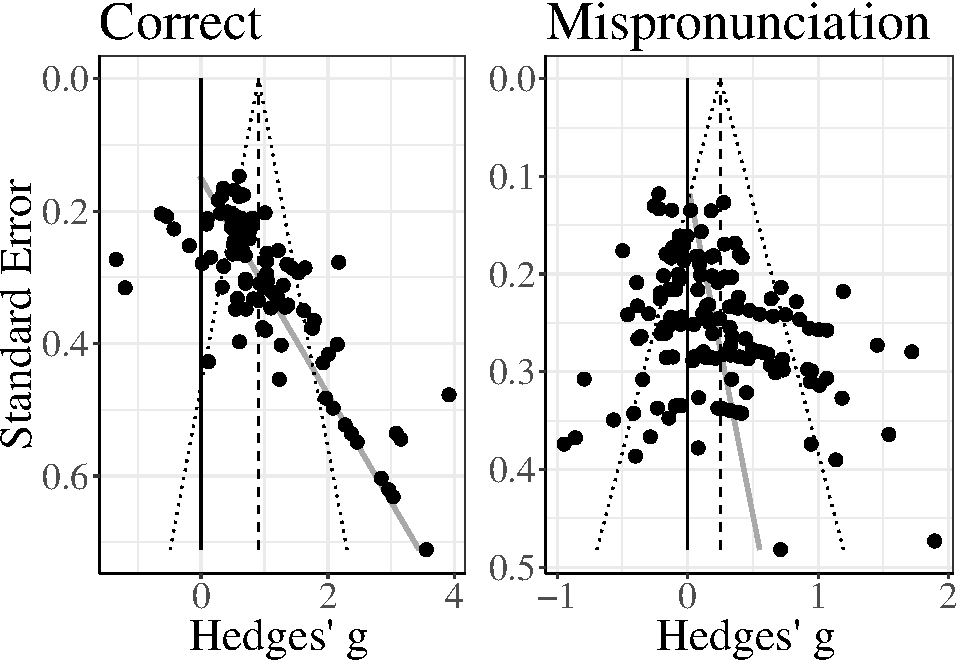
\includegraphics{Paper_Analyses_files/figure-latex/FunnelCombo-1.pdf}
\caption{}
\end{figure}

\begin{verbatim}
## [1] TRUE
\end{verbatim}

\begin{verbatim}
## [1] TRUE
\end{verbatim}

We next examined the p-curves for significant values from the correctly
pronounced and mispronounced conditions. The p-curve based on 72
statistically significant values for correct pronunciations indicates
that the data contain evidential value (Z = -17.93, \emph{p} \textless{}
.001) and there is no evidence of a large proportion of p-values just
below the typical alpha threshold of .05. The p-curve based on 36
statistically significant values for mispronunciations indicates that
the data contain evidential value (Z = -6.81, \emph{p} \textless{} .001)
and there is no evidence of a large proportion of p-values just below
the typical alpha threshold of .05.

{[}CHRISTINA: CAn you add the stats for the non-sig results?{]}{[}KATIE:
Are there stats that can be computed on the non-sig results? Or do you
just want an n for significant and non-significant studies?{]}

Taken together, the results suggest a tendency in the literature towards
publication bias. As a result, our meta-analysis may systematically
overestimate effect sizes and we therefore interpret all estimates with
caution. Yet, the p-curve analysis suggests that overall, the literature
contains evidential value, reflecting a \enquote{real} effect. We
therefore continue our meta-analysis.

\subsection{Meta-analysis}\label{meta-analysis-1}

\subsubsection{Object Identification for Correct and Mispronounced
Words}\label{object-identification-for-correct-and-mispronounced-words}

We first calculated the meta-analytic effect for object identification,
i.e.~looks to the target image in response to correctly pronounced
words. The variance-weighted meta-analytic effect size Hedges' \emph{g}
was 0.91 (SE = 0.12) which was significantly different from zero (95\%
CI {[}0.67, 1.14{]}, \emph{p} \textless{} .001). This is a rather large
effect size (according to the criteria set by Cohen, 1988; see also
Bergmann, et al., 2018; for comparative meta-analytic effect sizes in
language acquisition research). That the effect size is significantly
above zero suggests that when presented with the correctly pronounced
label, infants fixated the corresponding object. Our analysis of funnel
plot asymmetry, however, found evidence for publication bias, which
might lead to an overestimated effect sizes as smaller, non-significant
results might not be published. Although the effect size Hedges'
\emph{g} may be overestimated for object identification in response to
correctly pronounced words, the p-curve results and a CI lower bound of
0.67 suggests that this result is robust even when correcting for
publication bias. In other words, we are confident that the true
population mean lies above zero for object recognition of correctly
pronounced words.

{[}CHRISTINA: Can you explain what the CI lower bound means here? I
don't follow.{]}{[}KATIE: What do you think about this? The CI lower
bound stuff here actually comes from something you wrote, so tell me
whether its correct.{]}

We then calculated the meta-analytic effect for object identification in
response to mispronounced words. In this case, the variance-weighted
meta-analytic effect size Hedges' \emph{g} was 0.25 (SE = 0.06) which
was also significantly different from zero (95\% CI {[}0.13, 0.37{]},
\emph{p} \textless{} .001). This is considered a small effect size
(Cohen, 1988), but significantly above zero, which suggests that even
when presented with a mispronounced label, infants fixated the correct
object. In other words, infants are able to resolve mispronunciations, a
key skill in language processing We again note the publication bias
(which was smaller in this condition), and the possibility that the
effect size Hedges' \emph{g} may be overestimated. But, as the p-curve
indicated evidential value, we are confident in the overall patterns,
namely that infants fixate the target even after hearing a mispronounced
label.

Heterogeneity was significant for both correctly pronounced (Q(103) =
625.63, \emph{p} \textless{} .001) and mispronounced words, (Q(146) =
462.51, \emph{p} \textless{} .001). This indicated that the sample
contains unexplained variance leading to significant difference across
our studies beyond what is to be expected based on random sampling
error. We therefore continue with our moderator analysis.

\subsubsection{Mispronunciation Sensitivity Meta-analytic
Effect}\label{mispronunciation-sensitivity-meta-analytic-effect}

The above two analyses considered the data from mispronounced and
correctly pronounced words separately. To evaluate mispronunciation
sensitivity, we compared the effect size Hedges' \emph{g} for correct
pronunciations with mispronunciations directly, merging the two
datasets. The moderator test was significant, QM(1) = 215.76, \emph{p}
\textless{} .001. Hedges' \emph{g} for mispronunciation sensitivity was
0.50 (SE = 0.03), which indicated that the responses across conditions
were significantly different (95\% CI {[}0.43, 0.56{]}, \emph{p}
\textless{} .001). This confirms that although infants fixate the
correct object for both correct pronunciations and mispronunciations,
the observed fixations to target (as measured by the effect sizes) were
significantly greater for correct pronunciations. In other words, we
observe a significant difference between the two conditions and can now
quantify the modulation of fixation behavior in terms of standardized
effect sizes.

\subsubsection{Object Recognition and Mispronunciation Sensitivity
Modulated by
Age}\label{object-recognition-and-mispronunciation-sensitivity-modulated-by-age}

To evaluate the different predictions we laid out in the introduction
for how mispronunciation sensitivity will change as infants develop, we
next added the moderator age (centered, in days). In the first analyses,
we investigate the impact of age separately on conditions where words
were either pronounced correctly or not. Age did not significantly
modulate object identification in response to correctly pronounced
(QM(1) = 0.68, \emph{p} = 0.41) or mispronounced words (QM(1) = 1.72,
\emph{p} = 0.19). The lack of a significant modulation together with the
small estimates indicates that there was no relationship between age and
target looks in response to a correctly pronounced or mispronounced
label. This relationship is plotted in Figure 2.

{[}CHRISTINA{]} CAN YOU ADD ESTIMATES AND THEIR CIS?? Ideally everywhere
where you report a p-value {[}KATIE: Do you know how to calculate
Estimates and CIs for the Test of Moderators? Or do you mean reporting
the estimates and CIs even when the moderator test is not
significant?{]}

We then examined the interaction between age and mispronunciation
sensitivity (correct vs.~mispronounced words) in our whole dataset. The
moderator test was significant (QM(3) = 218.62, \emph{p} \textless{}
.001). This result is in line with the general observation that as
infants mature they become better at language processing. The
interaction between age and mispronunciation sensitivity, however, was
not significant \(\beta\) = 0.00, (SE = 0.01, 95\% CI {[}-0.01, 0.02{]},
\emph{p} = 0.731), suggesting that as infants age, their
mispronunciation sensitivity remains the same.

\subsection{Figure 2}\label{figure-2}

\begin{figure}[htbp]
\centering
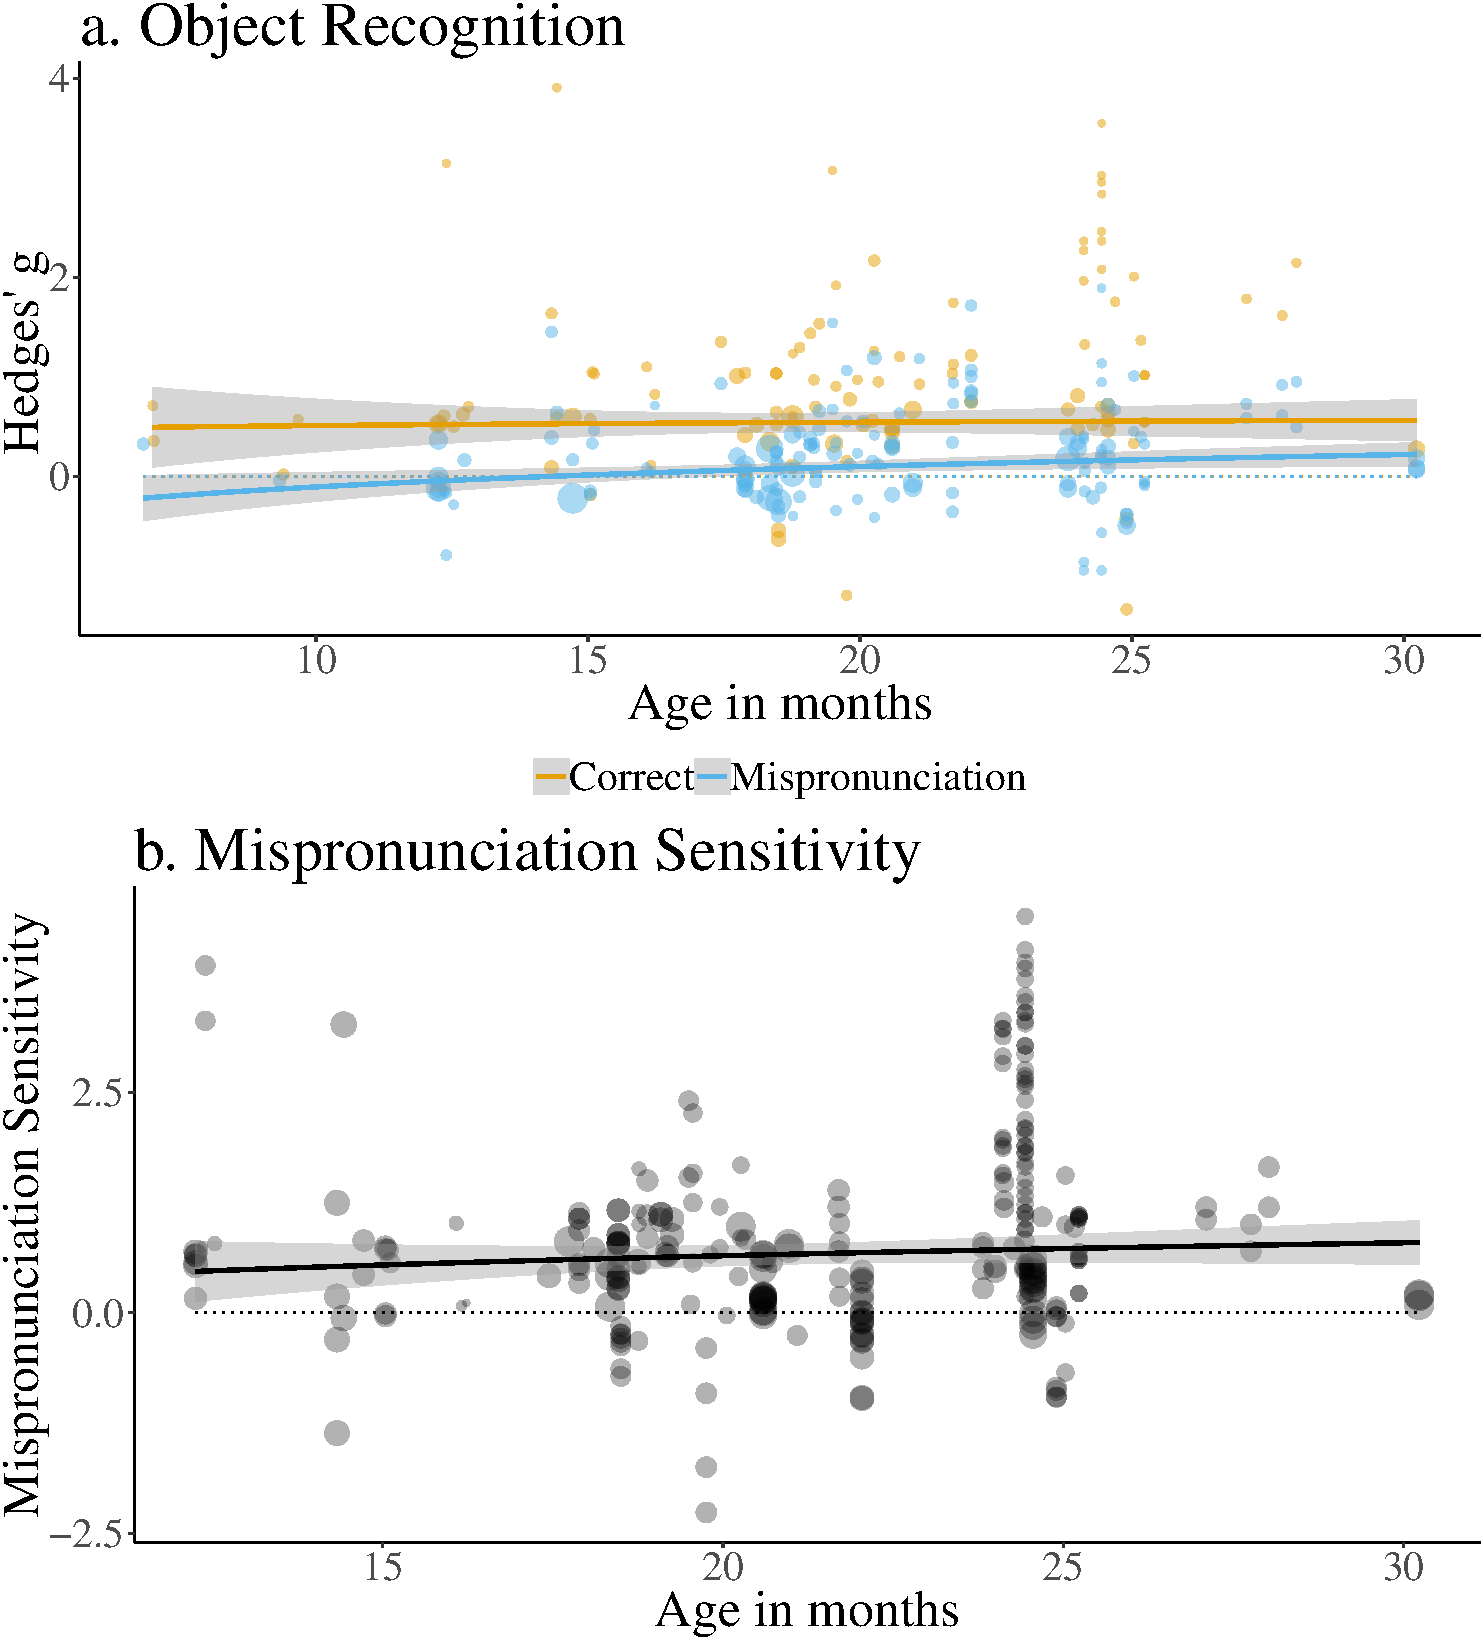
\includegraphics{Paper_Analyses_files/figure-latex/PlotMPEffect-1.pdf}
\caption{}
\end{figure}

\begin{verbatim}
## pdf 
##   2
\end{verbatim}

\subsubsection{Vocabulary Size: Correlation Between Mispronunciation
Sensitivity and
Vocabulary}\label{vocabulary-size-correlation-between-mispronunciation-sensitivity-and-vocabulary}

Of the 32 papers included in the meta-analysis, 8 (comprehension = 7
papers; production = 1) analyzed the relationship between vocabulary
scores and mispronunciation sensitivity. There is reason to believe that
production data are different from comprehension data (the former being
easier to estimate for parents in the typical questionnaire-based
assessment), so we analyze this data separately.

{[}KATIE{]} I DON'T KNOW HOW TO INTERPRET THESE RESULTS\ldots{} THE
FIXED EFFECTS MODEL ISN'T SIGNIFICANT FOR ANY OF THESE. IS THAT
MEANINGFUL? {[}CHRISTINA{]} SO WE DON'T WANT TO INTERPRET THE FIXED
EFFECTS MODEL AT ALL, IT IS NOT SUITABLE BECAUSE THERE IS VARIANCE
BETWEEN EVERY RECORD (LANGUAGE ETC). I WOULD INTERPRET THE OVERALL
CORRELATION AND THE CI, NOT THE P-VALUE (IN GENERAL). I ALSO WONDER
WHETHER WE SHOULD MOVE THE SUBSET ANALYSES TO THE SUPPLEMENTARY
MATERIALS AND JUST SAY OVERALL WE SEE NO RELATIONSHIPS AND CORRELATION
COEFFICIENTS CONSISTENYL BELOW .1 WE THEREFORE MUST CONCLUDE THAT WITHIN
NARROW AGE GROUPS VOCABULARY DOES NOT INFLUENCE ANYTHING WE LOOK AT. WE
CANNOT DO THIS ANALYSIS FPOR MP SENSITIVITY BECAUSE WE DON'T HAVE THE
NECESSARY RAW DATA. {[}KATIE: Ah, so because for each paper the
correlation and CI values straddle 0, this indicates that there really
isn't much evidence for a relationship? I think it could make sense to
add this to supplementary materials. Over the summer, I had also played
around with looking at how collection of vocabulary data has dropped off
over the years, even though more mispronunciation studies have been
published. That might be something interesting to add. If we truly think
that this is what is driving the development of mispronunciation
sensitivity, then why are people not collecting this data?{]} (BUT I
WONDER WHETHER WECOULD ENCODE THE REPORTED INTERACTION TERMS AND THE
CORRELATION AND THEN DO SOMETHING WITH THAT?) {[}KATIE: I'm not really
sure what you mean by this :({]}

\begin{verbatim}
##                                      COR            95%-CI %W(fixed)
## Zesiger et al. (2012)             0.0610 [-0.3553; 0.4773]       5.8
## Zesiger et al. (2012)            -0.1590 [-0.5663; 0.2483]       6.1
## Mani, Coleman, & Plunkett (2008)  0.0300 [-0.2271; 0.2871]      15.2
## Swingley & Aslin (2000)           0.1050 [-0.1564; 0.3664]      14.7
## Mani & Plunkett 2007             -0.1700 [-0.5234; 0.1834]       8.0
## Mani & Plunkett 2007             -0.1700 [-0.5175; 0.1775]       8.3
## Swingley & Aslin (2002)           0.1410 [-0.2432; 0.5252]       6.8
## Swingley & Aslin (2002)           0.1410 [-0.2596; 0.5416]       6.3
## Swingley 2003                     0.3400 [ 0.0470; 0.6330]      11.7
## Swingley 2003                     0.0600 [-0.3472; 0.4672]       6.1
## Hojen et al.                      0.2220 [-0.2591; 0.7031]       4.3
## Hojen et al.                      0.4820 [ 0.0935; 0.8705]       6.7
##                                  %W(random)
## Zesiger et al. (2012)                   6.2
## Zesiger et al. (2012)                   6.5
## Mani, Coleman, & Plunkett (2008)       13.7
## Swingley & Aslin (2000)                13.4
## Mani & Plunkett 2007                    8.3
## Mani & Plunkett 2007                    8.5
## Swingley & Aslin (2002)                 7.2
## Swingley & Aslin (2002)                 6.7
## Swingley 2003                          11.2
## Swingley 2003                           6.5
## Hojen et al.                            4.8
## Hojen et al.                            7.0
## 
## Number of studies combined: k = 12
## 
##                         COR            95%-CI    z p-value
## Fixed effect model   0.0897 [-0.0105; 0.1900] 1.75  0.0795
## Random effects model 0.0893 [-0.0212; 0.1999] 1.58  0.1132
## 
## Quantifying heterogeneity:
## tau^2 = 0.0060; H = 1.09 [1.00; 1.50]; I^2 = 15.7% [0.0%; 55.4%]
## 
## Test of heterogeneity:
##      Q d.f. p-value
##  13.05   11  0.2899
## 
## Details on meta-analytical method:
## - Inverse variance method
## - DerSimonian-Laird estimator for tau^2
## - Untransformed correlations
\end{verbatim}

\begin{verbatim}
##                                      COR            95%-CI %W(fixed)
## Zesiger et al. (2012)            -0.0090 [-0.4268; 0.4088]       5.0
## Zesiger et al. (2012)            -0.1720 [-0.5775; 0.2335]       5.3
## Mani, Coleman, & Plunkett (2008)  0.0700 [-0.1861; 0.3261]      13.2
## Mani & Plunkett 2007             -0.1100 [-0.4696; 0.2496]       6.7
## Mani & Plunkett 2007             -0.1100 [-0.4635; 0.2435]       6.9
## Swingley & Aslin (2002)           0.1820 [-0.1970; 0.5610]       6.0
## Swingley & Aslin (2002)           0.1820 [-0.2131; 0.5771]       5.6
## Swingley 2003                     0.1800 [-0.1406; 0.5006]       8.4
## Swingley 2003                     0.0700 [-0.3367; 0.4767]       5.2
## Ramon-Casas et al. 2009           0.0980 [-0.3068; 0.5028]       5.3
## Ramon-Casas et al. 2009          -0.1470 [-0.5468; 0.2528]       5.4
## Ramon-Casas et al. 2009          -0.2300 [-0.6171; 0.1571]       5.8
## Ramon-Casas et al. 2009           0.2400 [-0.1451; 0.6251]       5.9
## Ramon-Casas et al. 2009           0.4350 [ 0.1037; 0.7663]       7.9
## Hojen et al.                      0.2220 [-0.2591; 0.7031]       3.7
## Hojen et al.                     -0.1480 [-0.6430; 0.3470]       3.5
##                                  %W(random)
## Zesiger et al. (2012)                   5.0
## Zesiger et al. (2012)                   5.3
## Mani, Coleman, & Plunkett (2008)       13.2
## Mani & Plunkett 2007                    6.7
## Mani & Plunkett 2007                    6.9
## Swingley & Aslin (2002)                 6.0
## Swingley & Aslin (2002)                 5.6
## Swingley 2003                           8.4
## Swingley 2003                           5.2
## Ramon-Casas et al. 2009                 5.3
## Ramon-Casas et al. 2009                 5.4
## Ramon-Casas et al. 2009                 5.8
## Ramon-Casas et al. 2009                 5.9
## Ramon-Casas et al. 2009                 7.9
## Hojen et al.                            3.7
## Hojen et al.                            3.5
## 
## Number of studies combined: k = 16
## 
##                         COR            95%-CI    z p-value
## Fixed effect model   0.0601 [-0.0331; 0.1533] 1.26  0.2061
## Random effects model 0.0601 [-0.0331; 0.1533] 1.26  0.2061
## 
## Quantifying heterogeneity:
## tau^2 = 0; H = 1.00 [1.00; 1.42]; I^2 = 0.0% [0.0%; 50.7%]
## 
## Test of heterogeneity:
##      Q d.f. p-value
##  14.51   15  0.4870
## 
## Details on meta-analytical method:
## - Inverse variance method
## - DerSimonian-Laird estimator for tau^2
## - Untransformed correlations
\end{verbatim}

\begin{verbatim}
##                              COR             95%-CI %W(fixed) %W(random)
## Bailey & Plunkett (2002)  0.0630 [-0.3441;  0.4701]       2.5        2.7
## Bailey & Plunkett (2002) -0.0660 [-0.4729;  0.3409]       2.5        2.7
## Bailey & Plunkett (2002)  0.0630 [-0.3441;  0.4701]       2.5        2.7
## Bailey & Plunkett (2002) -0.0660 [-0.4729;  0.3409]       2.5        2.7
## Bailey & Plunkett (2002)  0.0630 [-0.3441;  0.4701]       2.5        2.7
## Bailey & Plunkett (2002) -0.0660 [-0.4729;  0.3409]       2.5        2.7
## Bailey & Plunkett (2002)  0.0630 [-0.3441;  0.4701]       2.5        2.7
## Bailey & Plunkett (2002) -0.0660 [-0.4729;  0.3409]       2.5        2.7
## Swingley (2009)          -0.1200 [-0.3715;  0.1315]       6.4        5.6
## Swingley (2009)           0.1300 [-0.1957;  0.4557]       3.8        3.8
## Swingley & Aslin (2000)   0.4210 [ 0.2036;  0.6384]       8.6        6.7
## Mani & Plunkett 2007     -0.0590 [-0.4349;  0.3169]       2.9        3.0
## Mani & Plunkett 2007     -0.0590 [-0.4349;  0.3169]       2.9        3.0
## Mani & Plunkett 2007     -0.1700 [-0.5234;  0.1834]       3.3        3.3
## Mani & Plunkett 2007     -0.1700 [-0.5175;  0.1775]       3.4        3.4
## Mani & Plunkett 2007      0.1000 [-0.2667;  0.4667]       3.0        3.2
## Mani & Plunkett 2007     -0.2800 [-0.6214;  0.0614]       3.5        3.5
## Mani & Plunkett 2007     -0.0700 [-0.3354;  0.1954]       5.8        5.2
## Mani & Plunkett 2007      0.1000 [-0.1641;  0.3641]       5.8        5.2
## Swingley & Aslin (2002)   0.1750 [-0.2050;  0.5550]       2.8        3.0
## Swingley & Aslin (2002)   0.1750 [-0.2212;  0.5712]       2.6        2.8
## Mani & Plunkett 2010     -0.3500 [-0.6640; -0.0360]       4.1        4.0
## Swingley 2003             0.1500 [-0.1738;  0.4738]       3.9        3.8
## Swingley 2003             0.1500 [-0.1738;  0.4738]       3.9        3.8
## Swingley 2003             0.0600 [-0.3472;  0.4672]       2.4        2.7
## Swingley 2003             0.0600 [-0.3472;  0.4672]       2.4        2.7
## Hojen et al.             -0.0510 [-0.5557;  0.4537]       1.6        1.8
## Hojen et al.              0.0510 [-0.4537;  0.5557]       1.6        1.8
## Hojen et al.              0.0600 [-0.4442;  0.5642]       1.6        1.8
## Hojen et al.             -0.0600 [-0.5642;  0.4442]       1.6        1.8
## Tao et al. 2012           0.5700 [ 0.1710;  0.9690]       2.6        2.7
## 
## Number of studies combined: k = 31
## 
##                         COR            95%-CI    z p-value
## Fixed effect model   0.0377 [-0.0260; 0.1014] 1.16  0.2465
## Random effects model 0.0322 [-0.0399; 0.1043] 0.87  0.3818
## 
## Quantifying heterogeneity:
## tau^2 = 0.0079; H = 1.11 [1.00; 1.39]; I^2 = 19.3% [0.0%; 48.4%]
## 
## Test of heterogeneity:
##      Q d.f. p-value
##  37.18   30  0.1719
## 
## Details on meta-analytical method:
## - Inverse variance method
## - DerSimonian-Laird estimator for tau^2
## - Untransformed correlations
\end{verbatim}

\begin{verbatim}
##                             COR             95%-CI %W(fixed) %W(random)
## Swingley (2009)          0.0700 [-0.1839;  0.3239]       6.4        5.4
## Swingley (2009)          0.1600 [-0.1628;  0.4828]       3.9        3.8
## Mani & Plunkett 2007    -0.2820 [-0.6292;  0.0652]       3.4        3.4
## Mani & Plunkett 2007    -0.2820 [-0.6292;  0.0652]       3.4        3.4
## Mani & Plunkett 2007    -0.1100 [-0.4696;  0.2496]       3.2        3.3
## Mani & Plunkett 2007    -0.1100 [-0.4635;  0.2435]       3.3        3.3
## Mani & Plunkett 2007     0.2300 [-0.1208;  0.5808]       3.3        3.4
## Mani & Plunkett 2007     0.2200 [-0.1325;  0.5725]       3.3        3.4
## Mani & Plunkett 2007    -0.2700 [-0.5173; -0.0227]       6.7        5.5
## Mani & Plunkett 2007    -0.0590 [-0.3248;  0.2068]       5.8        5.0
## Swingley & Aslin (2002)  0.0290 [-0.3627;  0.4207]       2.7        2.8
## Swingley & Aslin (2002)  0.0290 [-0.3793;  0.4373]       2.5        2.7
## Swingley (2016)         -0.2690 [-0.6326;  0.0946]       3.1        3.2
## Swingley (2016)         -0.2690 [-0.6326;  0.0946]       3.1        3.2
## Swingley (2016)         -0.2690 [-0.6326;  0.0946]       3.1        3.2
## Swingley (2016)         -0.2690 [-0.6326;  0.0946]       3.1        3.2
## Swingley (2016)         -0.2690 [-0.6326;  0.0946]       3.1        3.2
## Swingley (2016)         -0.2690 [-0.6326;  0.0946]       3.1        3.2
## Swingley 2003            0.1500 [-0.1738;  0.4738]       3.9        3.8
## Swingley 2003            0.1500 [-0.1738;  0.4738]       3.9        3.8
## Swingley 2003            0.0700 [-0.3367;  0.4767]       2.5        2.7
## Swingley 2003            0.0700 [-0.3367;  0.4767]       2.5        2.7
## Ramon-Casas et al. 2009  0.0980 [-0.3068;  0.5028]       2.5        2.7
## Ramon-Casas et al. 2009 -0.1470 [-0.5468;  0.2528]       2.6        2.7
## Ramon-Casas et al. 2009 -0.2300 [-0.6171;  0.1571]       2.7        2.9
## Ramon-Casas et al. 2009  0.2400 [-0.1451;  0.6251]       2.8        2.9
## Ramon-Casas et al. 2009  0.4350 [ 0.1037;  0.7663]       3.7        3.7
## Hojen et al.            -0.0510 [-0.5557;  0.4537]       1.6        1.8
## Hojen et al.             0.0510 [-0.4537;  0.5557]       1.6        1.8
## Hojen et al.             0.0790 [-0.4239;  0.5819]       1.6        1.9
## Hojen et al.            -0.0790 [-0.5819;  0.4239]       1.6        1.9
## 
## Number of studies combined: k = 31
## 
##                          COR            95%-CI     z p-value
## Fixed effect model   -0.0402 [-0.1043; 0.0238] -1.23  0.2181
## Random effects model -0.0393 [-0.1127; 0.0340] -1.05  0.2931
## 
## Quantifying heterogeneity:
## tau^2 = 0.0094; H = 1.13 [1.00; 1.42]; I^2 = 22.0% [0.0%; 50.1%]
## 
## Test of heterogeneity:
##      Q d.f. p-value
##  38.45   30  0.1386
## 
## Details on meta-analytical method:
## - Inverse variance method
## - DerSimonian-Laird estimator for tau^2
## - Untransformed correlations
\end{verbatim}

\subsubsection{Interim Discussion}\label{interim-discussion}

The main goal of this paper was to assess mispronunciation sensitivity
and its maturation with age. The results are clear: Although infants
consider a mispronunciation as a better match with the target image than
a distractor image, there was a consistent effect of mispronunciation
sensitivity. This did not change with development. Of the 3 predictions
and assumptions about the development of infants' sensitivity to
mispronunciations discussed in the Introduction, the present results
lend some support for the argument that mispronunciation sensitivity
stays consistent as infants develop. This runs counter to existing
theories of phono-lexical development, which predict either an increase
(PRIMR ref) or decrease (Assim Model ref) in mispronunciation
sensitivity.

{[}KATIE{]} CAN A CONCLUSION BE DRAWN FROM THE VOCABULARY RESULTS? IF
SO, THIS IS THE PARAGRAPH

In sum, it seems that current theories of infants' phono-lexical
development cannot fully capture our results and should be reconsidered
with all the evidence in mind.

Alternatively, the lack of developmental change in mispronunciation
sensitivity could be due to differences in the types of tasks given to
infants of different ages. To examine this possibility, we include an
exploratory analysis of whether different moderators and experimental
design features were included at different ages, in addition to
investigating the role that these moderators play in mispronunciation
sensitivity.

\subsection{Moderator Analyses}\label{moderator-analyses}

{[}cHRISTINA{]} I WOULD FOLLOW THE OUTLINE IN THE PREVIOUS PARAGRAPH
HERE OR FLIP THE PARAGRAPH AROUND: 1. ARE DIFFERENT MODERATORS USED AT
DIFFERENT AGES? TEST: sIMPLE CHI-SQUARED OF AGE GROUP VERSUS MODERATOR
ASSIGNMENT (AGE GROUP DETERMINED BY LOOKING AT THE YOUNGEST AGE FOR X?)
2. WHICH MODERATORS INFLUENCE MP SENSITIVITY TEST SIMPLE MA WITH
MODERATOR TESTS

OR \enquote{FOR EACH POSSIBLE MODERATOR WHICH COULD INFLIENCE MP
SENSITIVITY, WE FIRST TEST THIS POSSIBILITY AND THEN EVALUATE WHETHER
THERE IS A SYSTEMATIC DIFFERENCE OF MANIPULATING THESE MODERATORS AS
INFANTS MATURE, I.E. WHETHER OLDER INFANTS ARE TESTED ON A MORE
DIFFICULT TASK} ALSO, AS FINAL FOLLOW-UP IT WOULD BE PERFECT TO JUST
SUBSET ALL STUDIES WITH FAMILIAR DISTRACTORS, SAME NUMBER OF FEATURES,
AND CHECK THAT OUR CONCLUSIONS HOLD UP REGARING MP SENSITIVITY

{[}KATIE: I prefer this second option, first looking at the moderators
in general and then looking at whether there is this systematic
difference with age. The latter is exploratory, so I feel like this
information should not preceed our planned analyses.{]}

\subsubsection{Number of features
changed}\label{number-of-features-changed}

To assess whether the number of features changed modulates
mispronunciation sensitivity, we calculated the meta-analytic effect for
object identification in response to words that were pronounced
correctly and mispronounced using 1-, 2-, and 3-feature changes. We did
not include data for which the number of features changed in a
mispronunciation was not specified or the number of features changed was
not consistent (e.g., one mispronunciation included a 2-feature change
whereas another only a 1-feature change). This analysis was therefore
based on a subset of the overall dataset, with 81 experimental
conditions for correct pronunciations, 108 for 1-feature
mispronunciations, 16 for 2-feature mispronunciations, and 6 for
3-feature mispronunciations. Each feature change (from 0 to 3; 0
representing correct pronunciations) was considered to have an equal
impact on mispronunciation sensitivity, following the argument of graded
sensitivity (White \& Aslin, 2008; Mani \& Plunkett 2011).

To understand the relationship between number of features changed and
mispronunciation sensitivity, we evaluated the effect size Hedges'
\emph{g} with number of features changed as a moderator. The moderator
test was significant, QM(1) = 76.10, \emph{p} \textless{} .001. Hedges'
\emph{g} for number of features changed was -0.12 (SE = 0.01), which
indicated that as the number of features changed increased, the effect
size Hedges' \emph{g} significantly decreased (95\% CI {[}-0.15,
-0.10{]}, \emph{p} \textless{} .001). We plot this relationship in
Figure X. This confirms previous findings of a graded sensitivity to the
number of features changed for both consonant (White \& Morgan, 2008)
and vowel (Mani \& Plunkett, 2011) mispronunciations as well as the
importance of controlling for the degree of phonological mismatch in
experimental design.

\begin{figure}[htbp]
\centering
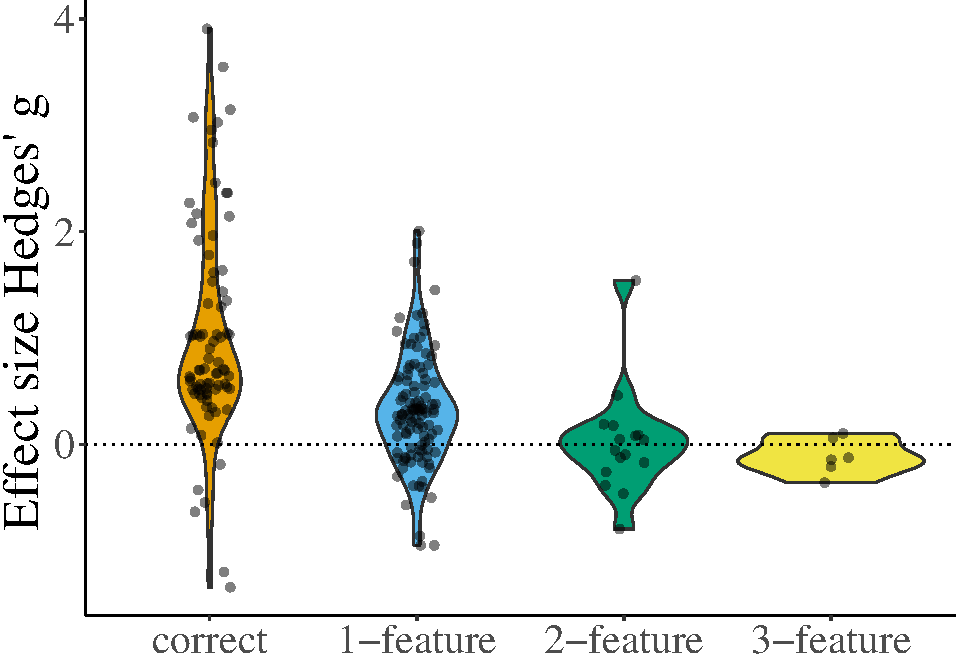
\includegraphics{Paper_Analyses_files/figure-latex/PlotFeatEffect-1.pdf}
\caption{}
\end{figure}

\begin{verbatim}
## pdf 
##   2
\end{verbatim}

Although we did not have any specific predictions about the relationship
between infant age and the impact of number of features changed on
mispronunciation sensitivity, we included an exploratory analysis to
examine this relationship. When age was also included as a moderator,
the moderator test was significant, QM(3) = 81.11, \emph{p} \textless{}
.001, but the interaction between age and number of features changed was
not significant, \(\beta\) = 0.01, (SE = 0.00, 95\% CI {[}0, 0.01{]},
\emph{p} = 0.069). This suggests that there is no relationship between
infant age the impact of number of features changed on mispronunciation
sensitivity.

Although all papers included in the dataset also included correct
pronunciations, not all papers included all three types of feature
changes (i.e.~1-3). The age range for each type of number of features
changed was 372.89 - 920.20 days (\emph{M} = 637.40) for 1-feature
mispronunciations, 377.28 - 920.20 days (\emph{M} = 612.17) for
2-feature mispronunciations, and 544.48 - 920.20 days (\emph{M} =
661.64) for 3-feature mispronunciations. Focusing on the ages where all
three numbers of features changed were tested (i.e.~544.48 - 920.20
days), however, did not change the pattern of results.

\subsubsection{Distractor familiarity}\label{distractor-familiarity}

We next assessed whether distractor familiarity has an impact on the
size of mispronunciation sensitivity. First, we calculated the
meta-analytic effect for object identification in response to
mispronounced target words/images that were paired with either a
familiar or an unfamiliar distractor image. The moderator test was not
significant QM(1) = 0.43, \emph{p} = 0.513. This suggests that upon
hearing a mispronunciation, infants looks to the target image were
similar for when the target image was paired with an image of a familiar
or unfamiliar object. We next assessed whether distractor familiarity
was related to mispronunciation sensitivity. We merged the two datasets
and included condition (correct pronunciation, mispronunciation) as an
additional moderator. The moderator test was significant, QM(3) =
219.46, \emph{p} \textless{} .001, but the interaction between
distractor familiarity and condition was not significant \(\beta\) =
0.14, (SE = 0.08, 95\% CI {[}-0.02, 0.30{]}, \emph{p} = 0.08). These
results suggest that overall, infants' familiarity with the distractor
object (familiar or unfamiliar) did not impact their mispronunciation
sensitivity.

\begin{figure}[htbp]
\centering
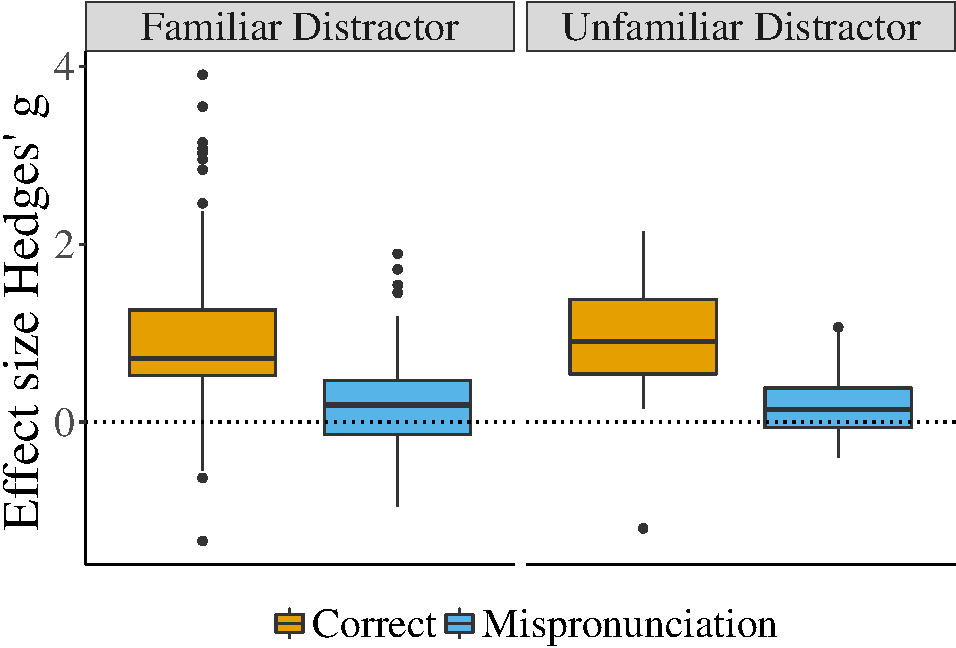
\includegraphics{Paper_Analyses_files/figure-latex/PlotDistFamEffect_NoAge-1.pdf}
\caption{}
\end{figure}

\begin{verbatim}
## pdf 
##   2
\end{verbatim}

We next examined whether age modulates object recognition or
mispronunciation sensitivity when the distractor image is familiar or
unfamiliar. For object recognition in response to a mispronunciation,
including age as a moderator resulted in a moderator test that was not
significant, QM(3) = 3.25, \emph{p} = 0.355. {[}CHRISTINA{]} I WORRY A
LOT AT THESE POINTS THAT THIS IS THE WHOLE P\textgreater{}.05 = NULL IS
TRUE FALLACY. WE CAN NEVER HAVE EVIDENCE FOR THE NULL HYPOTHESIS. SO
BETTER ITNERPRET ESTIMATES AND CIS.

This suggests that upon hearing a mispronunciation, infants looks to the
target image were similar for when the target image was paired with an
image of a familiar or unfamiliar object, regardless of their age. We
next assessed whether the relationship between distractor familiarity
and mispronunciation sensitivity was modulated by age. We merged the two
datasets and included condition (correct pronunciation,
mispronunciation) as well as age as additional moderators. The moderator
test was significant, QM(7) = 224.96, \emph{p} \textless{} .001.
Although the three-way-interaction between condition, distractor
familiarity, and age was not significant (\(\beta\) = -0.02, SE = 0.02,
95\% CI {[}-0.06, 0.02{]}, \emph{p} = 0.305), here the interaction
between condition and distractor familiarity was significant (\(\beta\)
= 0.18, SE = 0.09, 95\% CI {[}0, 0.35{]}, \emph{p} = 0.05).

{[}KATIE{]} WHAT DOES IT MEAN THAT IN THIS LAST TEST THERE WAS AN
INTERACTION BETWEEN CONDITION AND DISTRACTOR FAMILIARITY, WHEN AGE WAS
INCLUDED AS A MODERATOR? DOES THAT MEAN THAT AGE IS CONTROLLED FOR?
UNDERSTANDING THIS WILL HELP ME FORMULATE THE CONCLUSION SENTENCE AND
MOTIVATE THE NEXT SET OF ANALYSES.

{[}CHRISTINA{]} I WOULD NOT OVERINTERPRET IT, THE ESTIMATE DID NOT
DRAMATICALLY CHANGE, AND IT IS BARELY SIGNIFICANT. DOES THAT HELP?

{[}KATIE: I think so. I've just removed that part{]}

\begin{verbatim}
##                       Test                            Results
## 1 Welch Two Sample t-test: t(153.83) = 5.30, p < .001, d = NA
\end{verbatim}

Although we anticipated that older children may be more impacted by the
presence of a unfamiliar compared to familiar distractor image, we found
that age and distractor familiarity did not impact mispronunciation
sensitivity. Inspection of the ages tested using different kinds of
distractors, however, revealed differences. Infants tested using a
familiar distractor were younger (M = 588.76 days, SD = 136.47, range =
207.8 - 768 days) than those infants tested using an unfamiliar
distractor (M = 678.85 days, SD = 115.47, range = 544.48 - 920.2 days),
which a two-sample t-test revealed to be a significant difference,
t(153.83) = 5.30, p \textless{} .0001.

{[}CHRISTINA{]} CAN YOU TURN THE NUMBERS INTO R CODE HERE? aLSO, NOT
SURE WE NEED A T-TEST TO CONFIRM THE OBVIOUS.

{[}KATIE{]} SO, IS IT OKAY TO DO THE AGE SUBSET ANALYSIS AFTER THIS?
SOMETHING LIKE \enquote{TO ENSURE THAT THE LACK OF A DIFFERENCE WASN'T
DUE TO THE DIFFERENCE IN AGES OF INFANTS TESTED WITH DIFFERENT TYPES OF
DISTRACTORS, WE ANALYZED A SUBSET OF PAPERS THAT TESTED AGES WHERE BOTH
FAMILIAR AND UNFAMILIAR DISTRACTORS WERE USED.} IN THE SUBSET ANALYSIS,
FOR MISP SENSITIVITY, THERE IS A SIGNIFICANT INTERACTION BETWEEN
DISTRACTOR FAMILIARITY AND CONDITION.

{[}CHRISTINA{]} YES!!!!!!

\subsubsection{Phonological overlap between target and
distractor}\label{phonological-overlap-between-target-and-distractor}

To assess whether phonological overlap between the target and distractor
image labels has an impact on the size of mispronunciation sensitivity,
we examined the meta-analytic effect for object identification in
response to mispronunciations and mispronunciation sensitivity when the
target-distractor pairs either shared the same onset phoneme, had no
overlap, or where the distractor was an unfamiliar object. We did not
include data for which the overlap included both the onset and medial
phonemes (\emph{n} = 4) or coda phonemes (\emph{n} = 3). The analysis
was therefore based on a subset of the overall dataset, with 104
experimental conditions containing onset phoneme overlap between the
target and distractor, 80 containing no overlap between target and
distractor, and 60 for targets paired with unfamiliar distractor images.
There were therfore three possibilities for distractor overlap: onset
phoneme overlap, no overlap, and an unfamiliar distractor. In our
analysis, we were interested in the difference between overlap and lack
of overlap; therefore, experimental conditions containing onset phoneme
overlap were coded as the reference condition and compared with
responses to experimental conditions with no overlap or an unfamiliar
distractor separately.

{[}KATIE{]} CAN YOU CHECK THE WAY THAT I WROTE THE LAST SENTENCE?

{[}CHRISTINA{]} SEEMS OK BUT I AM CONFUSED WHY OVERLAP IS THE BASELINE
AND WHY YOU BRING IN NOVEL. I THINK YOU NEED TO SPELL THIS OUT MORE.

Regarding object identification in response to mispronunciations, when
distractor overlap was included as a moderator, the moderator test was
not significant QM(2) = 1.78, \emph{p} = 0.412. {[}CHRISTINA{]} AGAIN DO
NOT RELY ON P-VALUES BUT ON ESTIMATES AND CIS This suggests that upon
hearing a mispronunciation, infants looks to the target image were
similar for when the target image was paired with a distractor image
that contained overlap on the onset phoneme or no overlap with the
target word, or was an unfamiliar object. We next assessed whether
target-distractor overlap was related to mispronunciation sensitivity.
We merged the two datasets and included condition (correct
pronunciation, mispronunciation) as an additional moderator. The
moderator test was significant, QM(5) = 230.34, \emph{p} \textless{}
.001. The interaction between condition and target-distractor pairs with
no overlap was significant (\(\beta\) = -0.25, SE = 0.08, 95\% CI
{[}-0.40, -0.10{]}, \emph{p} = 0.001), suggesting that mispronunciation
sensitivity was greater when target-distractor pairs shared the same
onset phoneme compared to when they shared no phonological overlap. The
interaction between condition and target-distractor pairs with an
unfamiliar distractor was also significant (\(\beta\) = 0.19, SE = 0.09,
95\% CI {[}0.01, 0.37{]}, \emph{p} = 0.042), suggesting that
mispronunciation sensitivity was smaller when the distractor image
shared the same onset phoneme as the target image compared to when the
distractor image was an unfamiliar object. This can be seen in Figure X.

{[}christina{]} I THINK THESE SHOULD BE TWO SEPARATE ANALYSES\ldots{}
NOVEL IS CONCEPTUALLY DIFFERENT.

\begin{figure}[htbp]
\centering
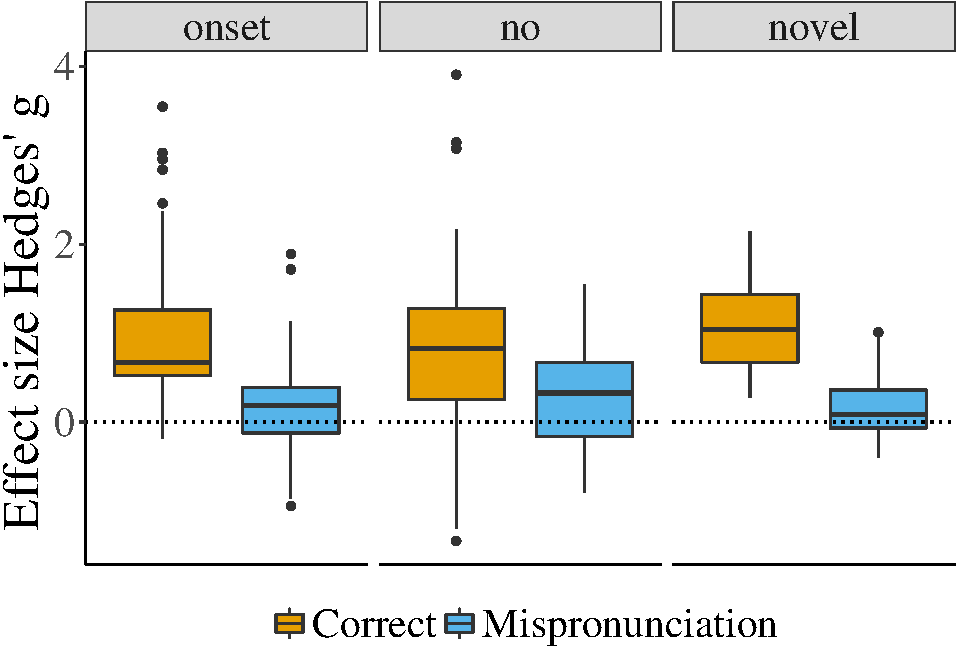
\includegraphics{Paper_Analyses_files/figure-latex/PlotDistOverlapEffect-1.pdf}
\caption{}
\end{figure}

\begin{verbatim}
## pdf 
##   2
\end{verbatim}

Although we did not have any specific predictions about the relationship
between infant age and the impact of distractor overlap on
mispronunciation sensitivity, we included an exploratory analysis to
examine this relationship. First, for object recognition in response to
mispronunciations, when age in addition to distractor overlap was also
included as a moderator, the moderator test was not significant, QM(5) =
5.99, \emph{p} = 0.308, suggesting that upon hearing a mispronunciation,
infants looks to the target image were similar for the three types of
overlap, regardless of infant age. We next assessed whether the
relationship between distractor overlap and mispronunciation sensitivity
was modulated by age. We merged the two datasets and included condition
(correct pronunciation, mispronunciation) as well as age as additional
moderators. The moderator test was significant, QM(11) = 243.40,
\emph{p} \textless{} .001. The interaction between age, condition, and
target-distractor pairs with no overlap was significant (\(\beta\) =
-0.04, SE = 0.02, 95\% CI {[}-0.08, 0.00{]}, \emph{p} = 0.032). As can
be seen in Figure X, the difference between correct pronunciations and
mispronunciations (mispronunciation sensitivity) stays steady across
infant ages for both target words paired with distractors containing
onset overlap with the target word as well as distractors containing no
overlap. As infants aged, however, overall recognition (regardless of
condition) increased for target-distractor pairs containing onset
overlap, whereas for overall recognition decreased for target-distractor
pairs containing no overlap. The interaction between age, condition, and
target-distractor pairs with an unfamiliar distractor was also
significant (\(\beta\) = -0.05, SE = 0.02, 95\% CI {[}-0.09, 0.00{]},
\emph{p} = 0.038). As can also be seen in Figure X, mispronunciation
sensitivity for target words paired with unfamiliar distractors
decreased with age, while it remained steady across a similar range of
ages for target words paired with distractors containing onset overlap
with the target word.

\begin{figure}[htbp]
\centering
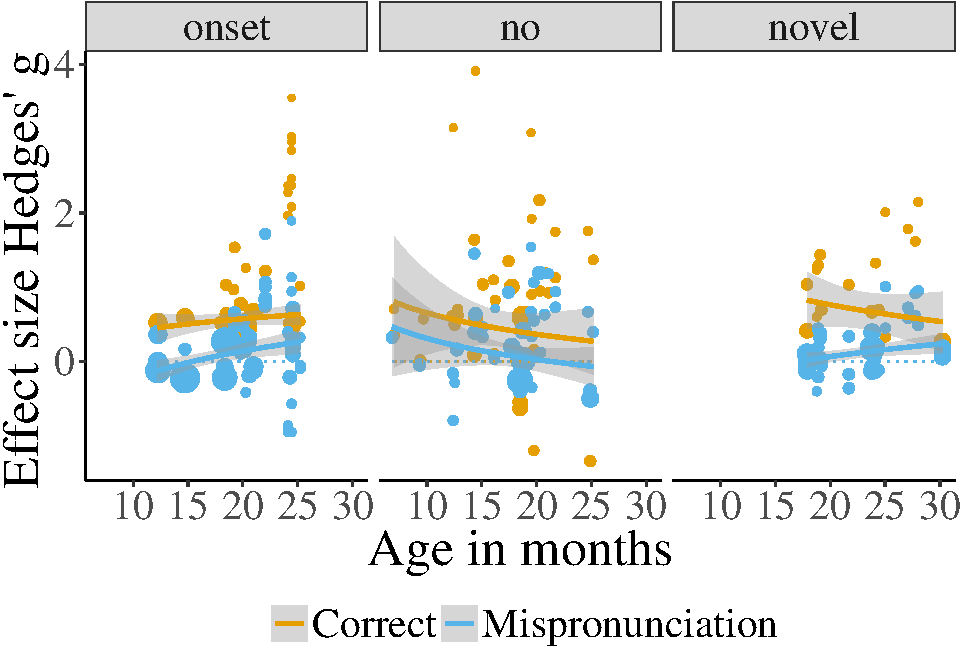
\includegraphics{Paper_Analyses_files/figure-latex/PlotDistOverlap_cond_age-1.pdf}
\caption{}
\end{figure}

\begin{verbatim}
## pdf 
##   2
\end{verbatim}

\subsubsection{Position of
mispronunciation}\label{position-of-mispronunciation}

To assess whether the position of the mispronunciation has an impact on
mispronunciation sensitivity, we calculated the meta-analytic effect for
object identification in response to mispronunciations on the onset and
medial phonemes. We did not include data for which the mispronunciation
was located on the coda (\emph{n} = 10 and NA), varied in regard to
position (\emph{n} = 3, 29, 8, and NA), or was not reported (\emph{n} =
10). The analysis was therefore based on a subset of the overall
dataset, with 143 and NA experimental conditions comparing a
mispronunciation on the onset phoneme and 48 and NA experimental
conditions comparing a mispronunciation on the medial phoneme.

Regarding object identification in response to mispronunciations, when
mispronunciation location was included as a moderator, the moderator
test was not significant QM(1) = 0.04, \emph{p} = 0.838. This suggests
that upon hearing a mispronunciation, infants looks to the target image
were similar for when the mispronunciation was located on the onset or
medial phonemes. We next assessed whether mispronunciation location was
related to mispronunciation sensitivity. We merged the two datasets and
included condition (correct pronunciation, mispronunciation) as an
additional moderator. The moderator test was significant, QM(3) =
180.76, \emph{p} \textless{} .001, but the interaction between
mispronunciation location and condition was not significant \(\beta\) =
0.05, (SE = 0.09, 95\% CI {[}-0.12, 0.22{]}, \emph{p} = 0.559). These
results suggest that overall, the location of the mispronunciation
(onset, medial) did not impact mispronunciation sensitivity.

\begin{figure}[htbp]
\centering
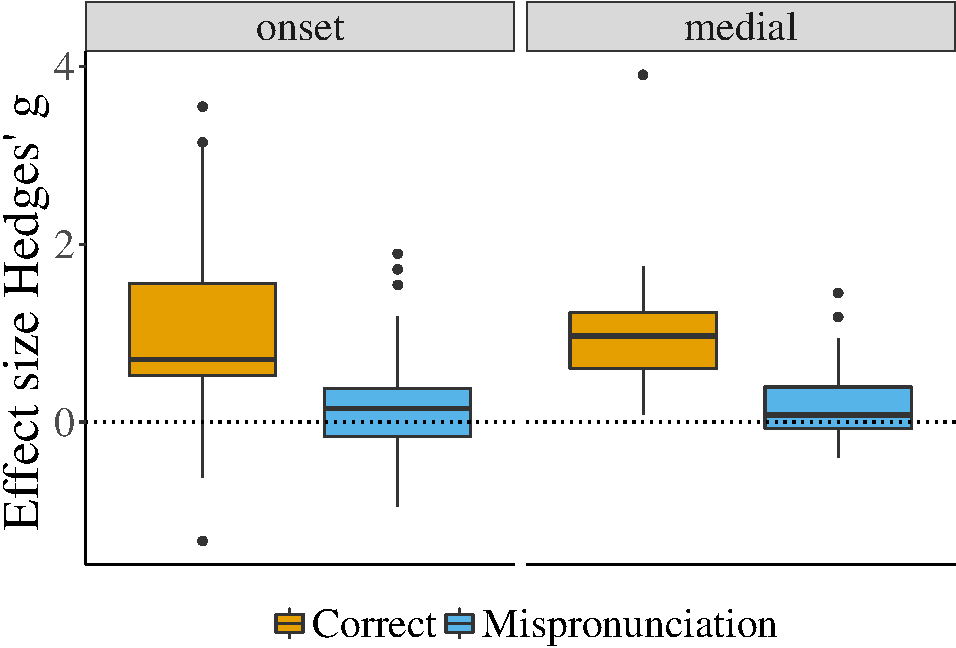
\includegraphics{Paper_Analyses_files/figure-latex/PlotPositionEffect-1.pdf}
\caption{}
\end{figure}

\begin{verbatim}
## pdf 
##   2
\end{verbatim}

Although we did not have any specific predictions about the relationship
between infant age and the impact of mispronuncition location on
mispronunciation sensitivity, we included an exploratory analysis to
examine this relationship. First, for object recognition in response to
mispronunciations, when age in addition to mispronunciation location was
also included as a moderator, the moderator test was not significant,
QM(3) = 1.22, \emph{p} = 0.747, suggesting that upon hearing a
mispronunciation, infants looks to the target image were similar for
both onset and medial mispronunciations, regardless of infant age. We
next assessed whether the relationship between mispronunciation location
and mispronunciation sensitivity was modulated by age. We merged the two
datasets and included condition (correct pronunciation,
mispronunciation) as well as age as additional moderators. The moderator
test was significant, QM(7) = 185.34, \emph{p} \textless{} .001, but the
interaction between mispronunciation location, age, and condition was
not significant \(\beta\) = NA, (SE = NA, 95\% CI {[}NA, NA{]}, \emph{p}
). These results provide further evidence that location of the
mispronunciation (onset, medial) did not impact mispronunciation
sensitivity.

\subsubsection{Type of mispronunciation (consonant or
vowel)}\label{type-of-mispronunciation-consonant-or-vowel}

To assess whether the type of mispronunciation impacts sensitivity to
mispronunciations, we calculated the meta-analytic effect for object
identification in response to the type of mispronunciation. Although
most theoretical discussion of mispronunciation type has focused on
consonants and vowels, our dataset also included tone mispronunciations.
In our analysis, we were interested in the difference between consonants
and vowels, but also include an exploratory analysis of responses to
tones, consonants, and vowels. We therefore conducted two sets of
analyses, one analyzing consonants and vowels alone and a second
comparing responses to tones with that of consonants and vowels,
separately. For the latter analysis, tones were coded as the reference
condition. We did not include data for which mispronunciation type
varied within experiment and was not reported separately (\emph{n} = 21
and 2). The analysis was therefore based on a subset of the overall
dataset, with 145 experimental conditions comparing a consonant
mispronunciation, 71 experimental conditions comparing a vowel
mispronunciation, and 12 experimental conditions comparing a tone
mispronunciation. Below, we first report the set of analyses comparing
consonants with vowels before moving on to the second set of exploratory
analyses comparing tones with that of consonants and vowels.

{[}KATIE{]} WHAT DO YOU THINK ABOUT THIS? WE HAVE THE TONES AND ITS A
NOVEL, INTERESTING THING, I THINK, AND PERHAPS WORTH IT TO INCLUDE A
COMPARISON OF TONES ALONGSIDE THE MORE THEORETICALLY IMPORTANT
COMPARISON BETWEEN CONSONANTS AND VOWELS.

We first analyzed experimental conditions where mispronunciation type
was either a consonant or vowel. Regarding object identification in
response to mispronunciations, when mispronunciation type was included
as a moderator, the moderator test was not significant QM(1) = 0.15,
\emph{p} = 0.702. This suggests that upon hearing a mispronunciation,
infants looks to the target image were similar for when the
mispronunciation was a consonant or a vowel. We next assessed whether
type of mispronunciation (consonant or vowel) was related to
mispronunciation sensitivity. We merged the two datasets and included
condition (correct pronunciation, mispronunciation) as an additional
moderator. The moderator test was significant, QM(3) = 145.14, \emph{p}
\textless{} .001, but the interaction between mispronunciation type and
condition was not significant \(\beta\) = 0.06, (SE = 0.08, 95\% CI
{[}-0.10, 0.21{]}, \emph{p} = 0.479). These results suggest that
overall, the type of mispronunciation (consonant vs.~vowel) did not
impact mispronunciation sensitivity.

We next examined whether age modulates object recognition or
mispronunciation sensitivity when the mispronunciation is a consonant or
vowel. For object recognition in response to a mispronunciation,
including age as a moderator resulted in a moderator test that was not
significant, QM(3) = 1.54, \emph{p} = 0.672. This suggests that upon
hearing a mispronunciation, infants looks to the target image were
similar for when the mispronunciation was on a consonant or vowel
phoneme, regardless of their age. We next assessed whether the
relationship between mispronunciation type (consonant or vowel) and
mispronunciation sensitivity was modulated by age. We merged the two
datasets and included condition (correct pronunciation,
mispronunciation) as well as age as additional moderators. The moderator
test was significant, QM(7) = 153.79, \emph{p} \textless{} .001. The
interaction between mispronunciation type, condition, and age was
significant (\(\beta\) = 0.04, SE = 0.02, 95\% CI {[}0.01, 0.08{]},
\emph{p} = 0.016). As can be seen in Figure X, as infants age,
mispronunciation sensitivity grows larger for vowel mispronunciations
but becomes smaller for consonant mispronunciations. Noticeably,
mispronunciation sensitivity appears greater for consonant compared to
vowel mispronunciations at younger ages, but this difference shifts as
infants age.

\begin{figure}[htbp]
\centering
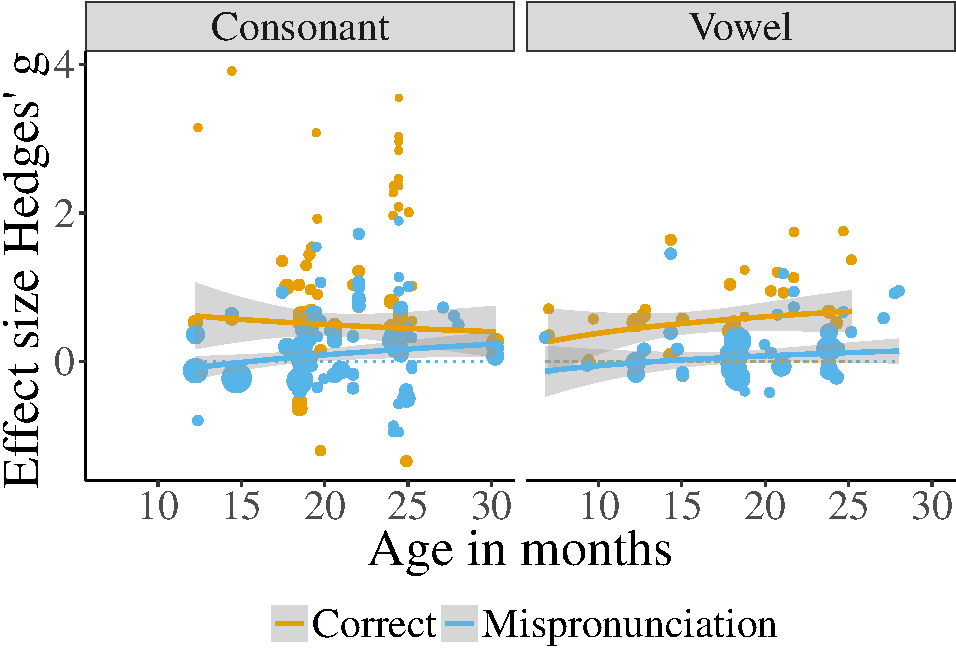
\includegraphics{Paper_Analyses_files/figure-latex/PlotCVEffect_cond_age-1.pdf}
\caption{}
\end{figure}

\begin{verbatim}
## pdf 
##   2
\end{verbatim}

To examine whether infants' native language impacts sensitivity to
consonant and vowel mispronunciations, we classified infants into
language families. Infants learning American English (\emph{n} = 56),
British English (\emph{n} = 66), Danish (\emph{n} = 6), Dutch (\emph{n}
= 58), and German (\emph{n} = 21) were classified into the Germanic
language family (\emph{n} = 207). Infants learning Catalan (\emph{n} =
4), Spanish (\emph{n} = 4), French (\emph{n} = 8), Catalan and Spanish
simultaneously (i.e.~bilinguals; \emph{n} = 6), and Swiss French
(\emph{n} = 6) were classified into the Romance language family
(\emph{n} = 28). For object recognition in response to a
mispronunciation, including language family as a moderator resulted in a
moderator test that was not significant, QM(3) = 5.36, \emph{p} = 0.147.
This suggests that upon hearing a mispronunciation, infants looks to the
target image were similar for when the mispronunciation was on a
consonant or vowel phoneme, regardless of the language family of their
native language. We next assessed whether the relationship between
mispronunciation type (consonant or vowel) and mispronunciation
sensitivity was modulated by language family. We merged the two datasets
and included condition (correct pronunciation, mispronunciation) as well
as language family as additional moderators. The moderator test was
significant, QM(7) = 158.89, \emph{p} \textless{} .001. The interaction
between condition and language family was significant (\(\beta\) = 0.73,
SE = 0.23, 95\% CI {[}0.27, 1.18{]}, \emph{p} = 0.002), suggesting
XXXXXXXXXXXXXX. The interaction between mispronunciation type,
condition, and language family was also significant (\(\beta\) = -0.87,
SE = 0.28, 95\% CI {[}-1.42, -0.32{]}, \emph{p} = 0.002). As can be seen
in Figure X, mispronunciation sensitivity for consonants was similar for
Germanic and Romance languages. Mispronunciation sensitivity for vowels,
however, was greater for Germanic compared to Romance languages.

{[}KATIE{]} I'M NOT REALLY SURE WHAT THE CONDITION BY LANGUAGE FAMILY
INTERACTION MEANS. SHOULD WE EVEN INTERPRET IT?

\begin{figure}[htbp]
\centering
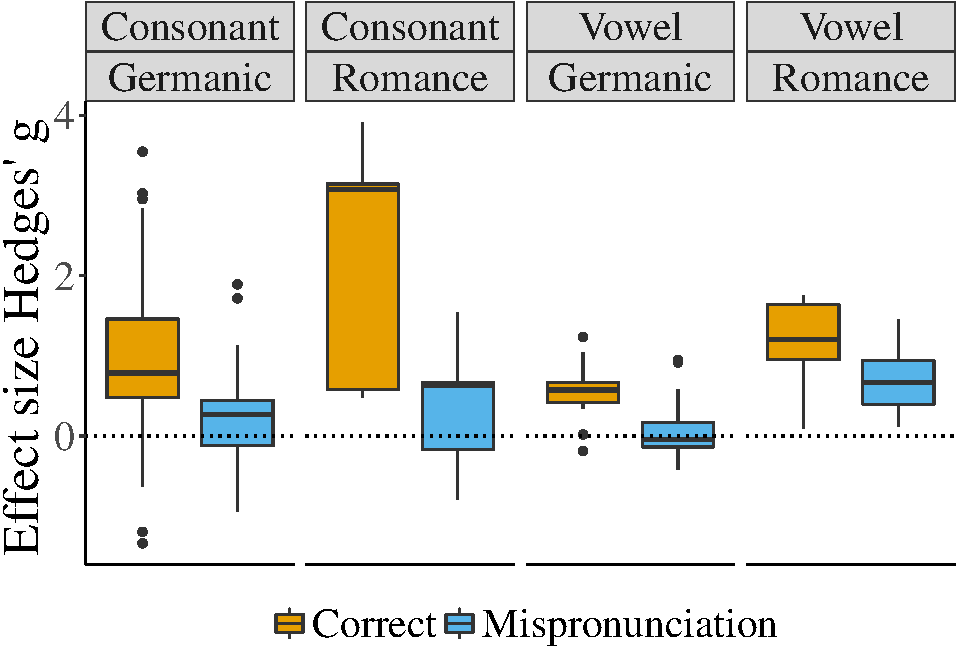
\includegraphics{Paper_Analyses_files/figure-latex/PlotCVEffect_Lang-1.pdf}
\caption{}
\end{figure}

\begin{verbatim}
## pdf 
##   2
\end{verbatim}

Finally, we examined the relationship between language family and infant
age and mispronunciation sensitivity to consonants and vowels. For
object recognition in response to a mispronunciation, including language
family and infant age as a moderator resulted in a moderator test that
was significant, QM(7) = 19.53, \emph{p} = 0.007. The interaction
between language family, age, and type of mispronunciation (consonant or
vowel) was significant, (\(\beta\) = 0.73, SE = 0.23, 95\% CI {[}0.27,
1.18{]}, \emph{p} = 0.002). As can be seen in Figure X, for infants
learning Germanic languages, increasing age was related to increasing
mispronunciation sensitivity for vowel mispronunciations, but decreasing
sensitivity for consonant mispronunciations. In contrast, infants
learning Romance languages have an even greater increase with age in
sensitivity to vowel mispronunciations. Surprisingly, sensitivity to
consonant mispronunciations shows a reversal in infants learning Romance
languages: the growth in target looks for consonant mipronunciations
increases and surpases that of target looks for correct pronunciations.

{[}KATIE{]} AGAIN, THERE ARE ADDITIONAL INTERACTIONS THAT ARE
SIGNIFICANT\ldots{} SHOULD THEY BE INTERPRETED? ALSO, WTF ROMANCE
LANGUAGES?

\begin{figure}[htbp]
\centering
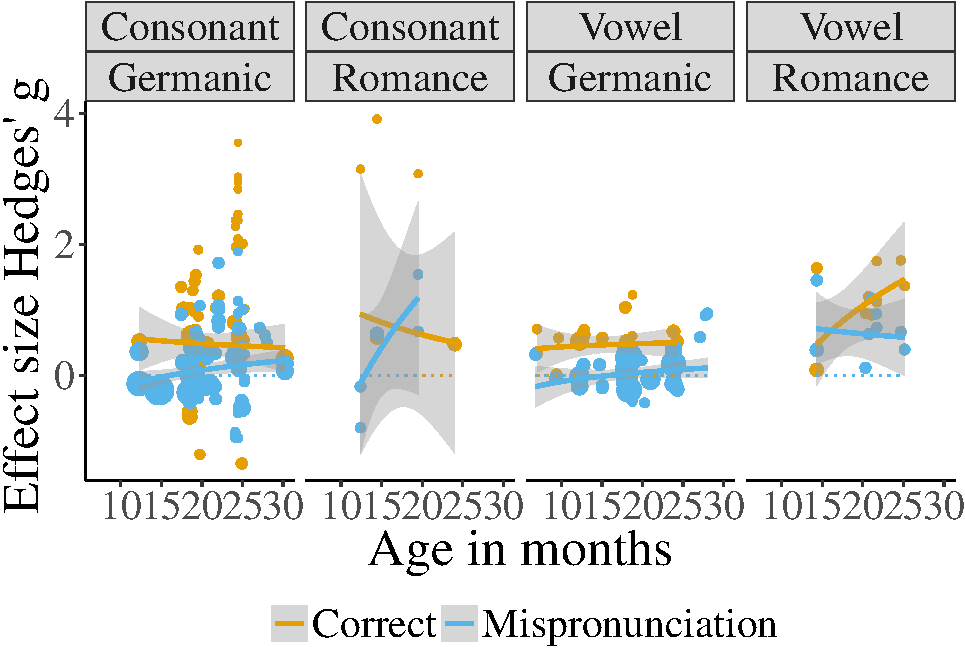
\includegraphics{Paper_Analyses_files/figure-latex/PlotCVEffect_cond_age_fam-1.pdf}
\caption{}
\end{figure}

\begin{verbatim}
## pdf 
##   2
\end{verbatim}

Although we had no predictions regarding mispronunciation sensitivity to
tone mispronunciations, we included an exploratory analysis to examine
whether responses to tone mispronunciations were different from that of
consonants or vowels. Regarding object identification in response to
mispronunciations, when mispronunciation type was included as a
moderator, the moderator test was not significant QM(2) = 1.16, \emph{p}
= 0.56. This suggests that upon hearing a mispronunciation, infants
looks to the target image were similar for tone mispronunciations in
comparison with both consonants and vowels. We next assessed whether
type of mispronunciation (tone, consonant, vowel) was related to
mispronunciation sensitivity. We merged the two datasets and included
condition (correct pronunciation, mispronunciation) as an additional
moderator. The moderator test was significant, QM(5) = 154.88, \emph{p}
\textless{} .001. The interaction between condition and consonant
mispronunciations was not significant \(\beta\) = -0.19, (SE = 0.21,
95\% CI {[}-0.59, 0.21{]}, \emph{p} = 0.359), suggesting that there was
no difference in looks to the target in response to consonant and tone
mispronunciations. The interaction between condition and vowel
mispronunciations was also not significant \(\beta\) = -0.13, (SE =
0.21, 95\% CI {[}-0.55, 0.28{]}, \emph{p} = 0.528), suggesting that
there was no difference in looks to the target in response to vowel and
tone mispronunciations.

We further included an exploratory analysis of the relationship between
infant age and the impact of tone mispronunciations in comparison to
consonant and vowel mispronunciations. First, for object recognition in
response to mispronunciations, when age in addition to mispronunciation
location was also included as a moderator, the moderator test was not
significant, QM(5) = 2.78, \emph{p} = 0.733. This suggests that upon
hearing a mispronunciation, infants looks to the target image were not
different between tone and vowel or tone and consonant
mispronunciations, regardless of their age. We next assessed whether the
relationship between mispronunciation type (tone, consonant, vowel) and
mispronunciation sensitivity was modulated by age. We merged the two
datasets and included condition (correct pronunciation,
mispronunciation) as well as age as additional moderators. The moderator
test was significant, QM(11) = 163.85, \emph{p} \textless{} .001, but
the interactions between condition, age, and both consonant
mispronciations (\(\beta\) = 0.02, SE = 0.10, 95\% CI {[}-0.19, 0.22{]},
\emph{p} = 0.871) and vowel mispronunciations (\(\beta\) = 0.06, SE =
0.10, 95\% CI {[}-0.14, 0.27{]}, \emph{p} = 0.56) were not significant.
Infants' sensitivity to tone mispronunciations compared to consonant or
vowel mispronunciations did not differ with age.

{[}KATIE{]} WORTH IT TO INCLUDE LANGUAGE FAMILY ANALYSES TOO?

\section{Discussion}\label{discussion}

To Summarize:

** Overall Meta-analytic Effect **

\begin{itemize}
\tightlist
\item
  Accept mispronunciations as labels for targets
\item
  Sensitive to mispronunciations
\item
  lack of change over development
\end{itemize}

** Vocabulary **

\begin{itemize}
\tightlist
\item
  no relationship?
\item
  talk about how few studies report it
\end{itemize}

** Size of Mispronunciation **

\begin{itemize}
\tightlist
\item
  graded sensitivity to number of features changed in a mispronunciation
\item
  importance for controlling in experimental design
\item
  Perhaps a call for more studies to include multiple number of features
  changed, so that this can be assessed? There was a narrow age where
  this was actually manipulated.
\end{itemize}

** Distractor Familiarity **

\begin{itemize}
\tightlist
\item
  Not really sure, check the results. A key interaction is significant
  in one model but not the other.
\item
  Again, ages not matched very well for the two groups here. Decide
  about whether to include a age subset analysis
\end{itemize}

** Phonological overlap between target and distractor **

\begin{itemize}
\tightlist
\item
  mispronunciation sensitivity was greater when target-distractor pairs
  shared the same onset phoneme compared to when they shared no
  phonological overlap
\item
  this is rather the opposite of what one would expect, right?
\item
  mispronunciation sensitivity was smaller when the distractor image
  shared the same onset phoneme as the target image compared to when the
  distractor image was an unfamiliar object
\item
  Maybe it would be useful to have time course analyses to address this
  issue further
\item
  As infants aged, overall recognition (regardless of condition)
  increased for target-distractor pairs containing onset overlap,
  whereas overall recognition decreased for target-distractor pairs
  containing no overlap.
\item
  mispronunciation sensitivity for target words paired with unfamiliar
  distractors decreased with age, while it remained steady across a
  similar range of ages for target words paired with distractors
  containing onset overlap with the target word.
\end{itemize}

** Position of mispronunciation **

\begin{itemize}
\tightlist
\item
  really no impact at all
\end{itemize}

** Type of mispronunciation **

\begin{itemize}
\tightlist
\item
  Overall, no difference between consonants and vowels
\item
  Consonant mispronunciation sensitivity decreases with age
\item
  Vowel mispronunciation sensitivity increases with age
\item
  mispronunciation sensitivity for consonants similar for Germanic and
  Romance languages
\item
  Mispronunciation sensitivity for vowels greater for Germanic compared
  to Romance languages
\item
  For Germanic infants, increasing age was related to increasing
  mispronunciation sensitivity for vowel mispronunciations, but
  decreasing sensitivity for consonant mispronunciations.
\item
  For Romance infants, an even greater increase with age in sensitivity
  to vowel mispronunciations.
\item
  For Romance infants, the growth in target looks for consonant
  mipronunciations increases and surpases that of target looks for
  correct pronunciations
\item
  exploratory analyses with tone mispronunciations suggest no great
  difference in sensitivity when compared to consonant and vowel
  mispronunciations
\end{itemize}

When it comes to designing studies, best practices and current standards
might not always overlap. Indeed, across a set of previous meta-analyses
it was shown that particularly infant research does not adjust sample
sizes according to the effect in question (Bergmann et al., in press). A
meta-analysis is a first step in improving experiment planning by
measuring the underlying effect and its variance, which is directly
related to the sample needed to achieve satisfactory power in the null
hypothesis significance testing framework. Failing to take effect sizes
into account can both yield to underpowered research and to testing too
many participants, both consequences are undesirable for a number of
reasons that have been discussed in depth elsewhere. We will just
briefly mention two that we consider most salient for theory building:
Underpowered studies will lead to false negatives more frequently than
expected, which in turn results in an unpublished body of literature
(citationcitation). Overpowered studies mean that participants were
tested unnecessarily, which has substantial ethical consequences
particularly when working with infants and other difficult to recruit
and test populations.

From Christina: let's make a note to put sth in the discussion about our
curve being surprisingly flat for correctly pronounced words bc people
adapt their analysis windows? Bc if you look at Molly's reaction time
paper, there is a steep increase.

Discussing the Moderator Analyses Maybe put them together into the ones
that worked out as we predicted and those that didn't? So, here is
evidence that supports existing arguments, that doesn't need to be a
huge chunk. But then more space devoted to moderator analyses that
didn't work out according to predictions.

It should be noted that the majority of consonant mispronunciations were
located on the onset phoneme (\emph{n} = 120; total consonant
conditions, \emph{n} = 145), while the majority of vowel
mispronunciations were located on the medial phoneme (\emph{n} = 44;
total vowel conditions, \emph{n} = 71). In their analysis using TRACE,
Mayor and Plunkett (2014) found that the difference between sensitivity
to consonant and vowel mispronunciations was due to infants' lexical
knowlege consisting of a majority consonant onset words.

{[}KATIE{]} COME BACK TO THIS.

\newpage

\section{References}\label{references}

\begingroup
\setlength{\parindent}{-0.5in} \setlength{\leftskip}{0.5in}

\hypertarget{refs}{}

\endgroup


\end{document}
